\documentclass[11pt]{article}
\usepackage[textwidth=18.0cm, textheight=23.0cm, top=2.0cm]{geometry}
\usepackage{pst-all}
\usepackage{amssymb}
\usepackage{tikz}
\usepackage{underscore}\begin{document}
\pagestyle{empty}


ClassName: \underline{\textbf{Class_08.2bp-33}}
\par
BinSize: \underline{\textbf{100 × 100}}
\par
ReduceSize: \underline{\textbf{100 × 100}}
\par
TypeNum: \underline{\textbf{80}}
\par
Num: \underline{\textbf{80}}
\par
OutS: \underline{\textbf{200000}}
\par
InS: \underline{\textbf{171793}}
\par
Rate: \underline{\textbf{0.859}}
\par
UB: \underline{\textbf{20}}
\par
LB0: \underline{\textbf{20}}
\par
LB: \underline{\textbf{20}}
\par
LBWithCut: \underline{\textbf{20}}
\par
NodeCut: \underline{\textbf{0}}
\par
ExtendedNodeCnt: \underline{\textbf{1}}
\par
GenNodeCnt: \underline{\textbf{1}}
\par
PrimalNode: \underline{\textbf{0}}
\par
ColumnCount: \underline{\textbf{20}}
\par
TotalCutCount: \underline{\textbf{0}}
\par
RootCutCount: \underline{\textbf{0}}
\par
LPSolverCnt: \underline{\textbf{1}}
\par
PricingSolverCnt: \underline{\textbf{0}}
\par
BranchAndBoundNum: \underline{\textbf{1}}
\par
isOpt: \underline{\textbf{true}}
\par
TimeOnInitSolution: \underline{\textbf{0.230 s}}
\par
TimeOnPrimal: \underline{\textbf{0.000 s}}
\par
TimeOnPricing: \underline{\textbf{0.000 s}}
\par
TimeOnRmp: \underline{\textbf{0.078 s}}
\par
TotalTime: \underline{\textbf{0.355 s}}
\par
\newpage


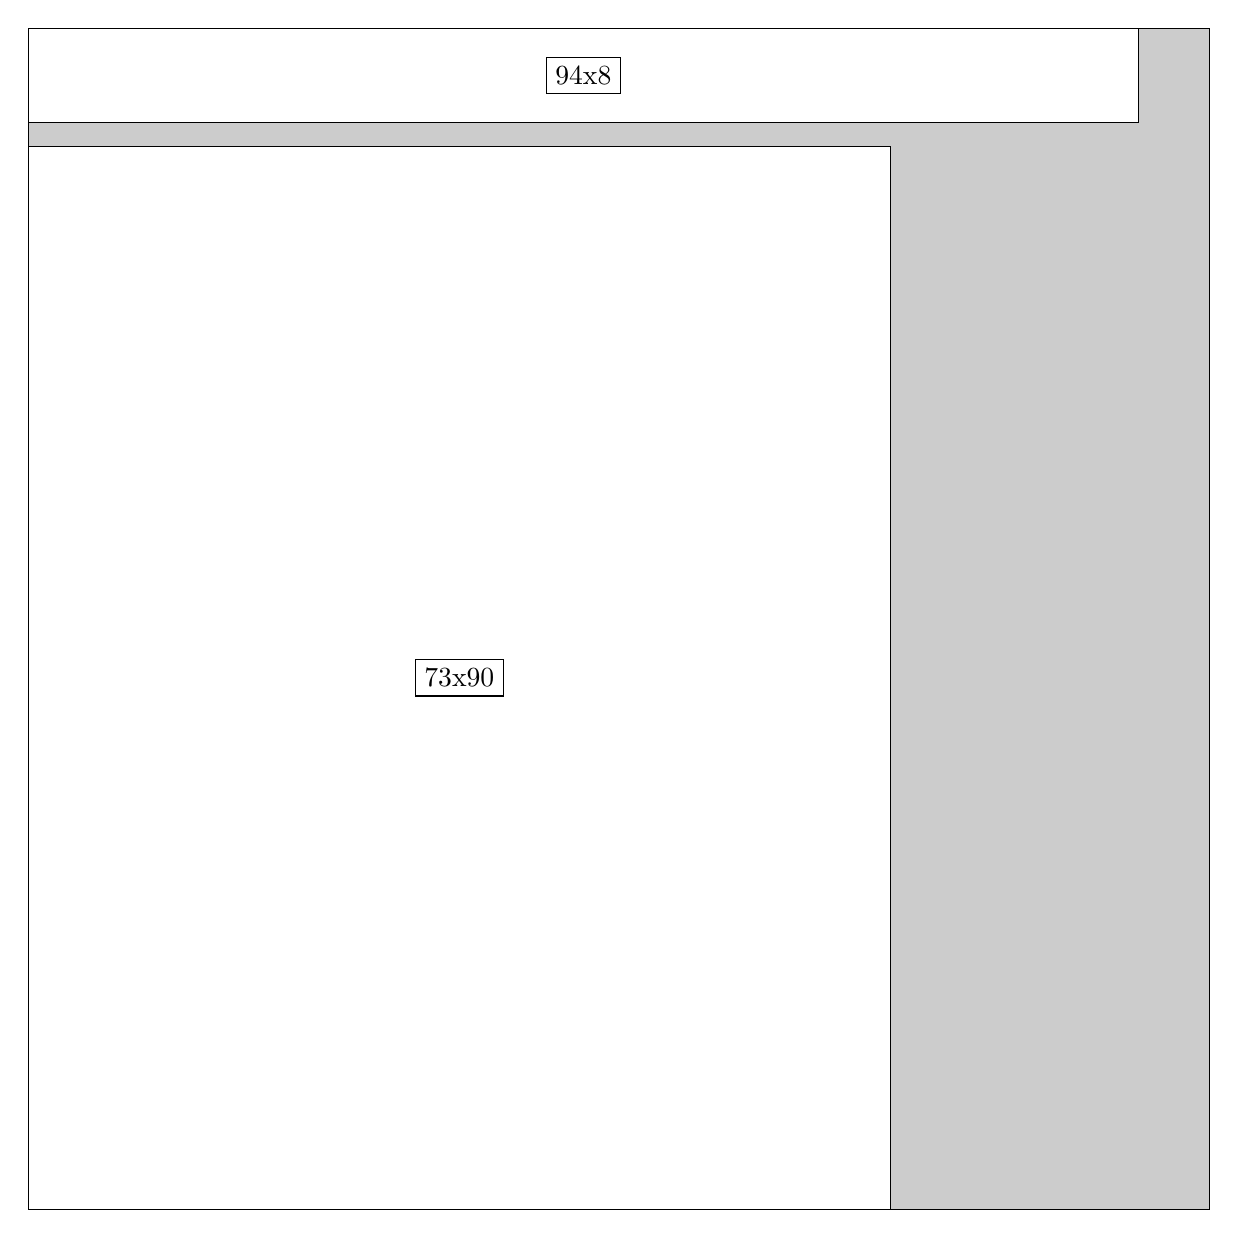
\begin{tikzpicture}[shorten >=1pt,scale=1.0,every node/.style={scale=1.0},->]
\tikzstyle{vertex}=[circle,fill=black!25,minimum size=14pt,inner sep=0pt]
\filldraw[fill=gray!40!white, draw=black] (0,0) rectangle (15.0,15.0);
\foreach \name/\x/\y/\w/\h in {73x90/0.0/0.0/10.95/13.5,94x8/0.0/13.799999999999999/14.1/1.2}
\filldraw[fill=white!40!white, draw=black] (\x,\y) rectangle node[draw] (\name) {\name} ++(\w,\h);
\end{tikzpicture}


w =73 , h =90 , x =0 , y =0 , v =6570
\par
w =94 , h =8 , x =0 , y =92 , v =752
\par
\newpage


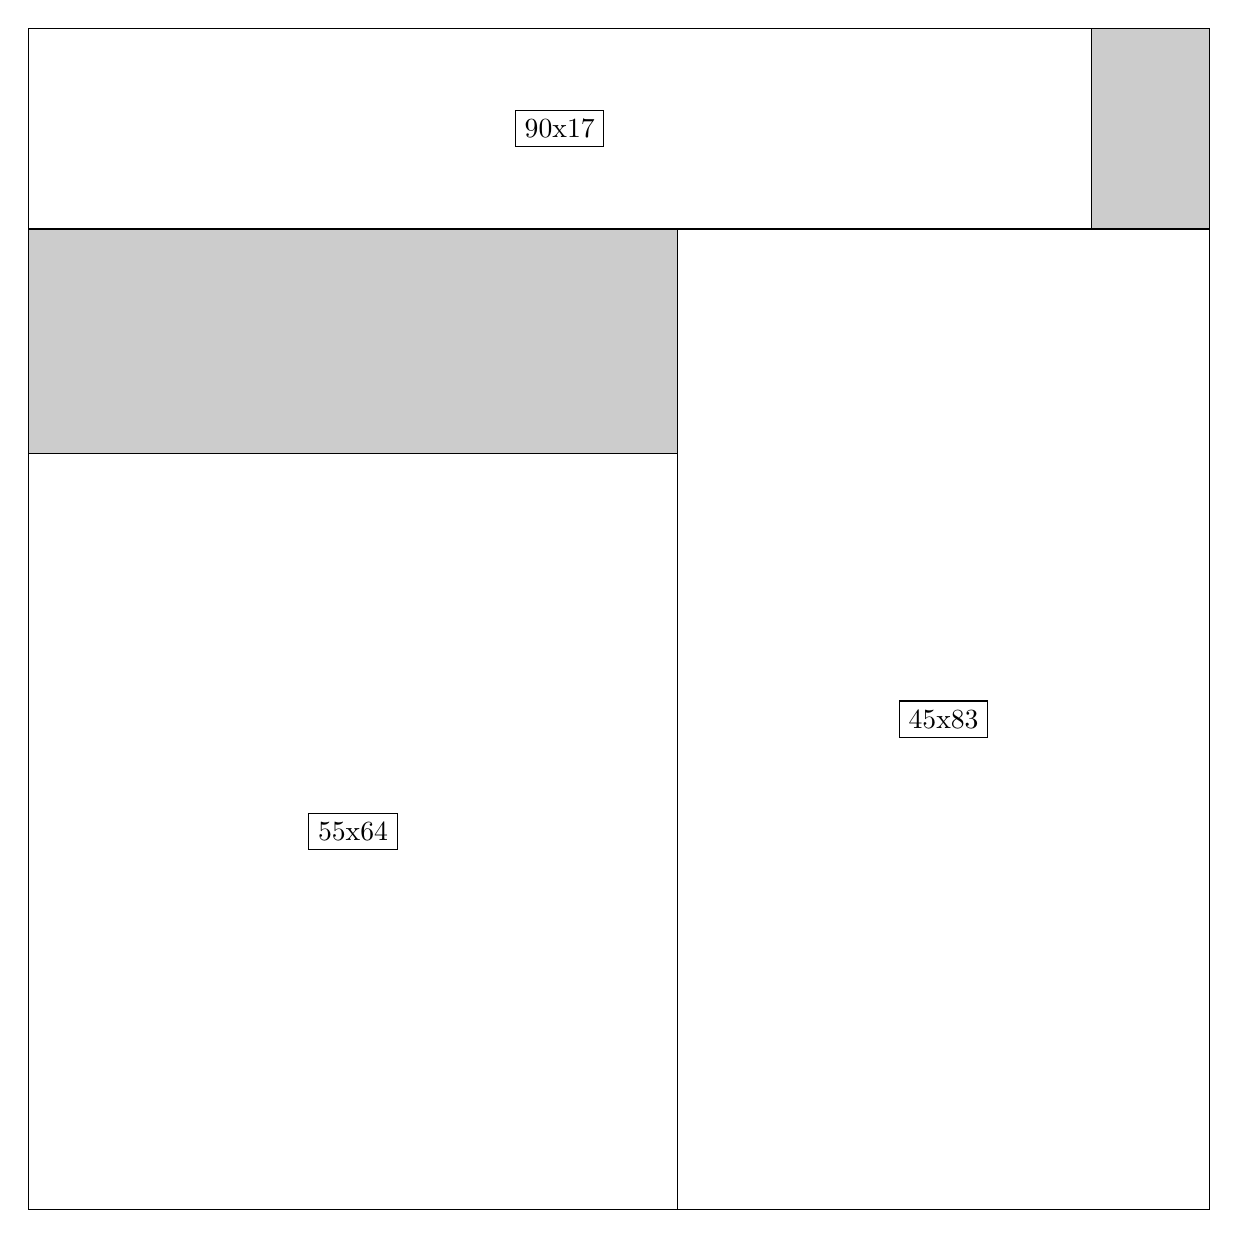
\begin{tikzpicture}[shorten >=1pt,scale=1.0,every node/.style={scale=1.0},->]
\tikzstyle{vertex}=[circle,fill=black!25,minimum size=14pt,inner sep=0pt]
\filldraw[fill=gray!40!white, draw=black] (0,0) rectangle (15.0,15.0);
\foreach \name/\x/\y/\w/\h in {55x64/0.0/0.0/8.25/9.6,45x83/8.25/0.0/6.75/12.45,90x17/0.0/12.45/13.5/2.55}
\filldraw[fill=white!40!white, draw=black] (\x,\y) rectangle node[draw] (\name) {\name} ++(\w,\h);
\end{tikzpicture}


w =55 , h =64 , x =0 , y =0 , v =3520
\par
w =45 , h =83 , x =55 , y =0 , v =3735
\par
w =90 , h =17 , x =0 , y =83 , v =1530
\par
\newpage


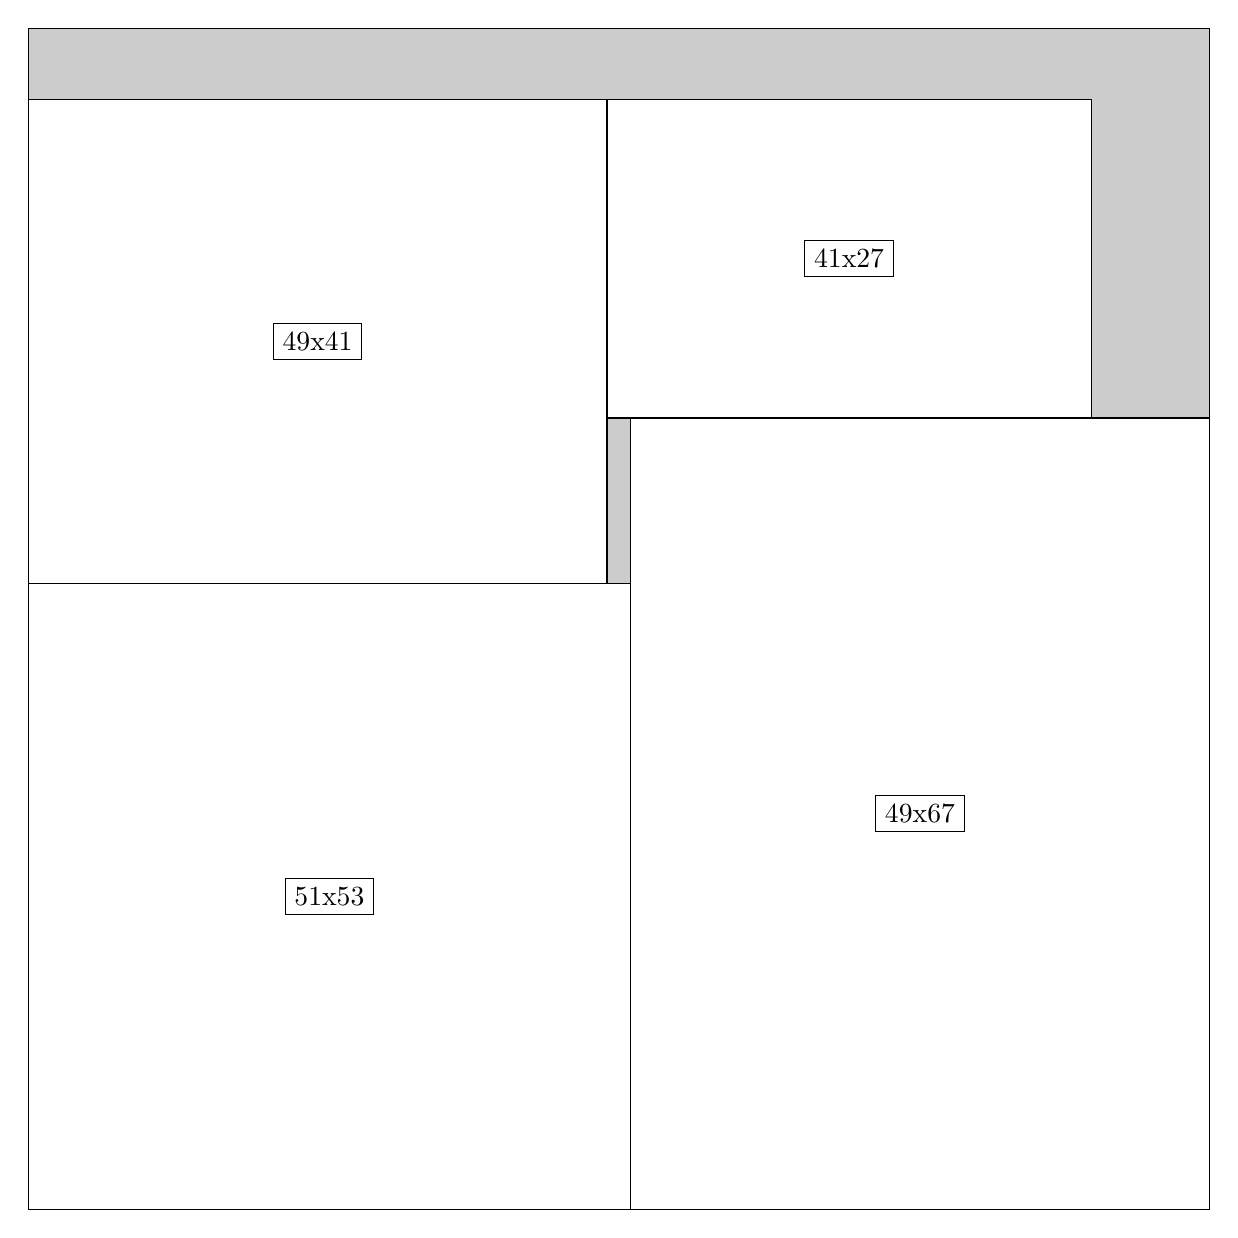
\begin{tikzpicture}[shorten >=1pt,scale=1.0,every node/.style={scale=1.0},->]
\tikzstyle{vertex}=[circle,fill=black!25,minimum size=14pt,inner sep=0pt]
\filldraw[fill=gray!40!white, draw=black] (0,0) rectangle (15.0,15.0);
\foreach \name/\x/\y/\w/\h in {49x67/7.6499999999999995/0.0/7.35/10.049999999999999,51x53/0.0/0.0/7.6499999999999995/7.949999999999999,49x41/0.0/7.949999999999999/7.35/6.1499999999999995,41x27/7.35/10.049999999999999/6.1499999999999995/4.05}
\filldraw[fill=white!40!white, draw=black] (\x,\y) rectangle node[draw] (\name) {\name} ++(\w,\h);
\end{tikzpicture}


w =49 , h =67 , x =51 , y =0 , v =3283
\par
w =51 , h =53 , x =0 , y =0 , v =2703
\par
w =49 , h =41 , x =0 , y =53 , v =2009
\par
w =41 , h =27 , x =49 , y =67 , v =1107
\par
\newpage


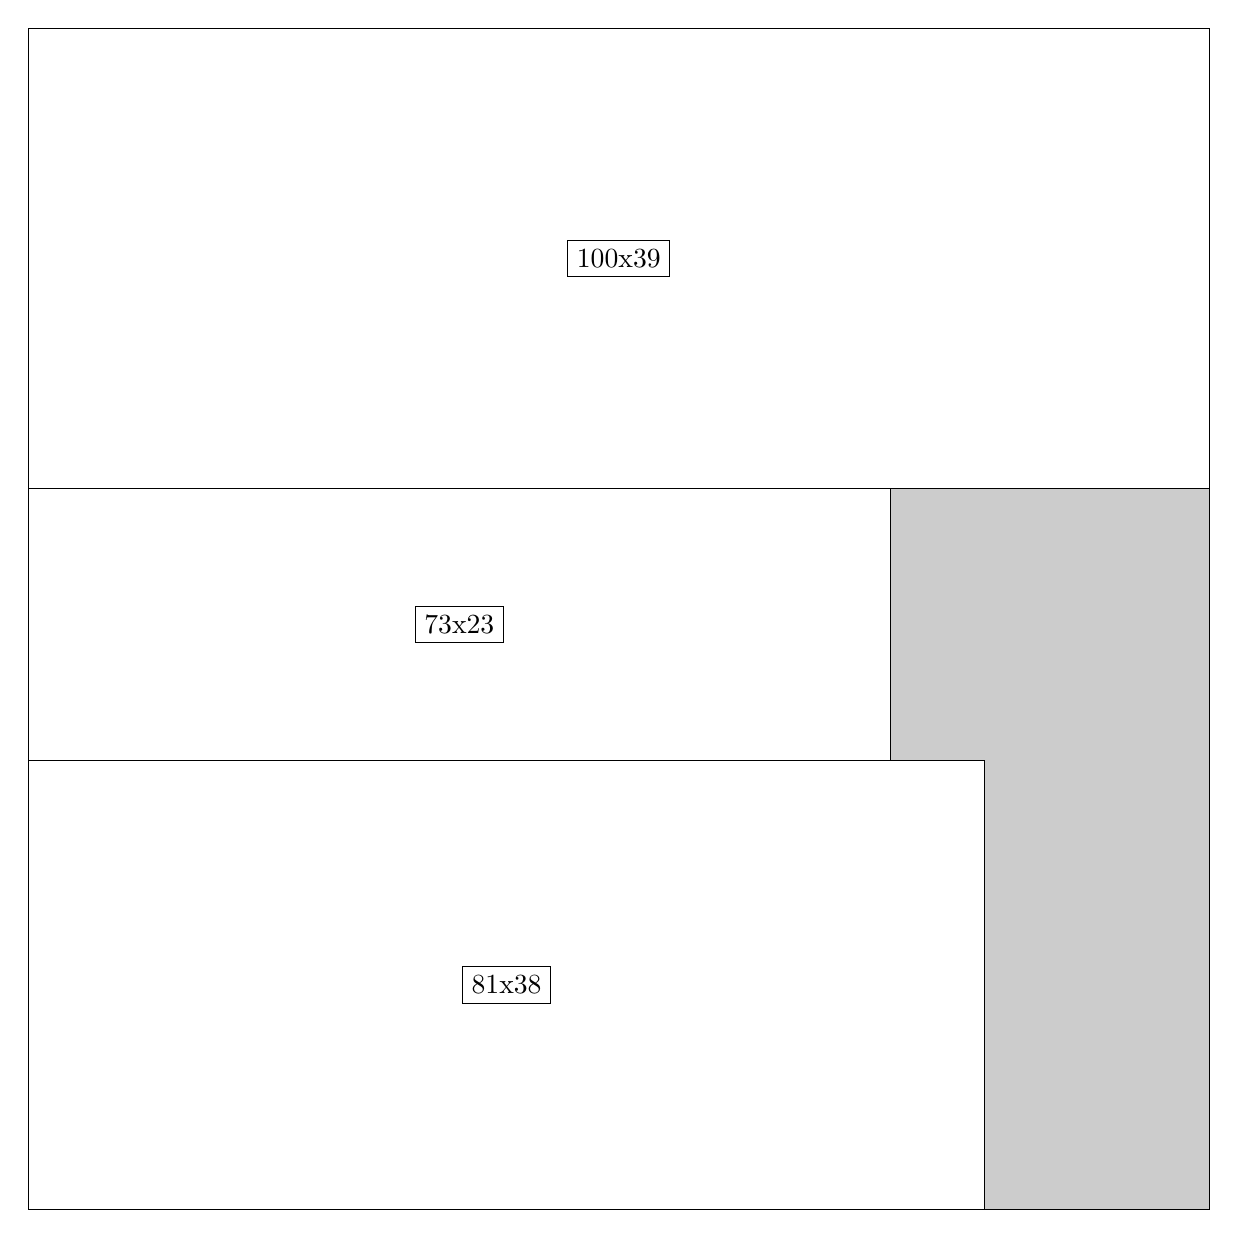
\begin{tikzpicture}[shorten >=1pt,scale=1.0,every node/.style={scale=1.0},->]
\tikzstyle{vertex}=[circle,fill=black!25,minimum size=14pt,inner sep=0pt]
\filldraw[fill=gray!40!white, draw=black] (0,0) rectangle (15.0,15.0);
\foreach \name/\x/\y/\w/\h in {100x39/0.0/9.15/15.0/5.85,81x38/0.0/0.0/12.15/5.7,73x23/0.0/5.7/10.95/3.4499999999999997}
\filldraw[fill=white!40!white, draw=black] (\x,\y) rectangle node[draw] (\name) {\name} ++(\w,\h);
\end{tikzpicture}


w =100 , h =39 , x =0 , y =61 , v =3900
\par
w =81 , h =38 , x =0 , y =0 , v =3078
\par
w =73 , h =23 , x =0 , y =38 , v =1679
\par
\newpage


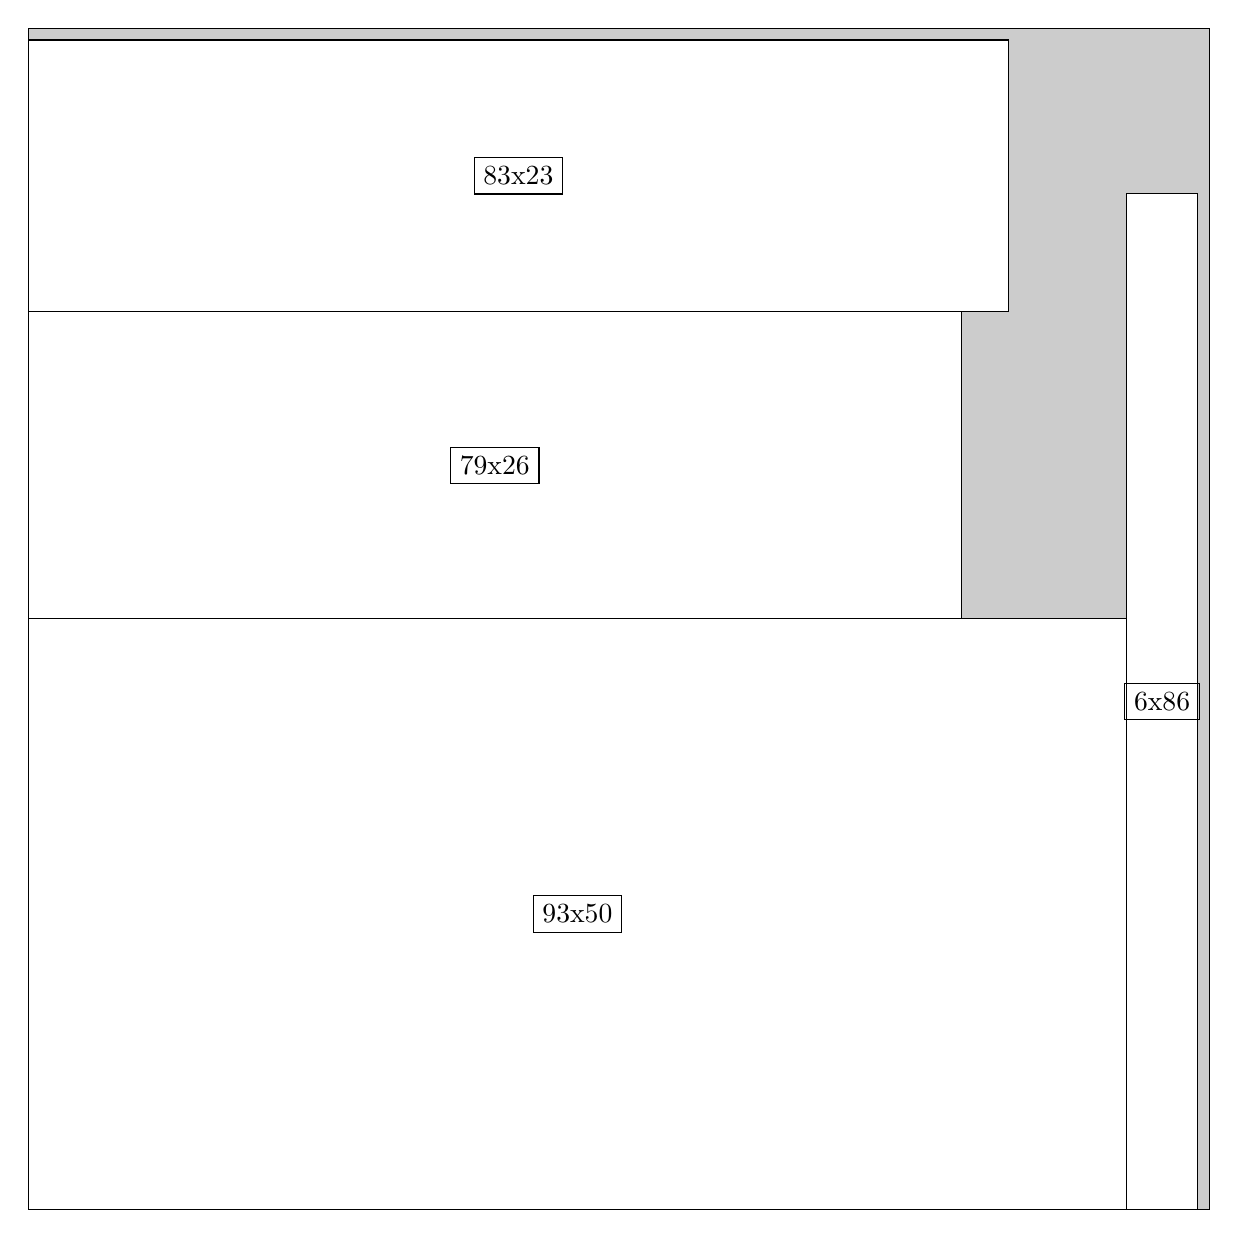
\begin{tikzpicture}[shorten >=1pt,scale=1.0,every node/.style={scale=1.0},->]
\tikzstyle{vertex}=[circle,fill=black!25,minimum size=14pt,inner sep=0pt]
\filldraw[fill=gray!40!white, draw=black] (0,0) rectangle (15.0,15.0);
\foreach \name/\x/\y/\w/\h in {93x50/0.0/0.0/13.95/7.5,79x26/0.0/7.5/11.85/3.9,83x23/0.0/11.4/12.45/3.4499999999999997,6x86/13.95/0.0/0.8999999999999999/12.9}
\filldraw[fill=white!40!white, draw=black] (\x,\y) rectangle node[draw] (\name) {\name} ++(\w,\h);
\end{tikzpicture}


w =93 , h =50 , x =0 , y =0 , v =4650
\par
w =79 , h =26 , x =0 , y =50 , v =2054
\par
w =83 , h =23 , x =0 , y =76 , v =1909
\par
w =6 , h =86 , x =93 , y =0 , v =516
\par
\newpage


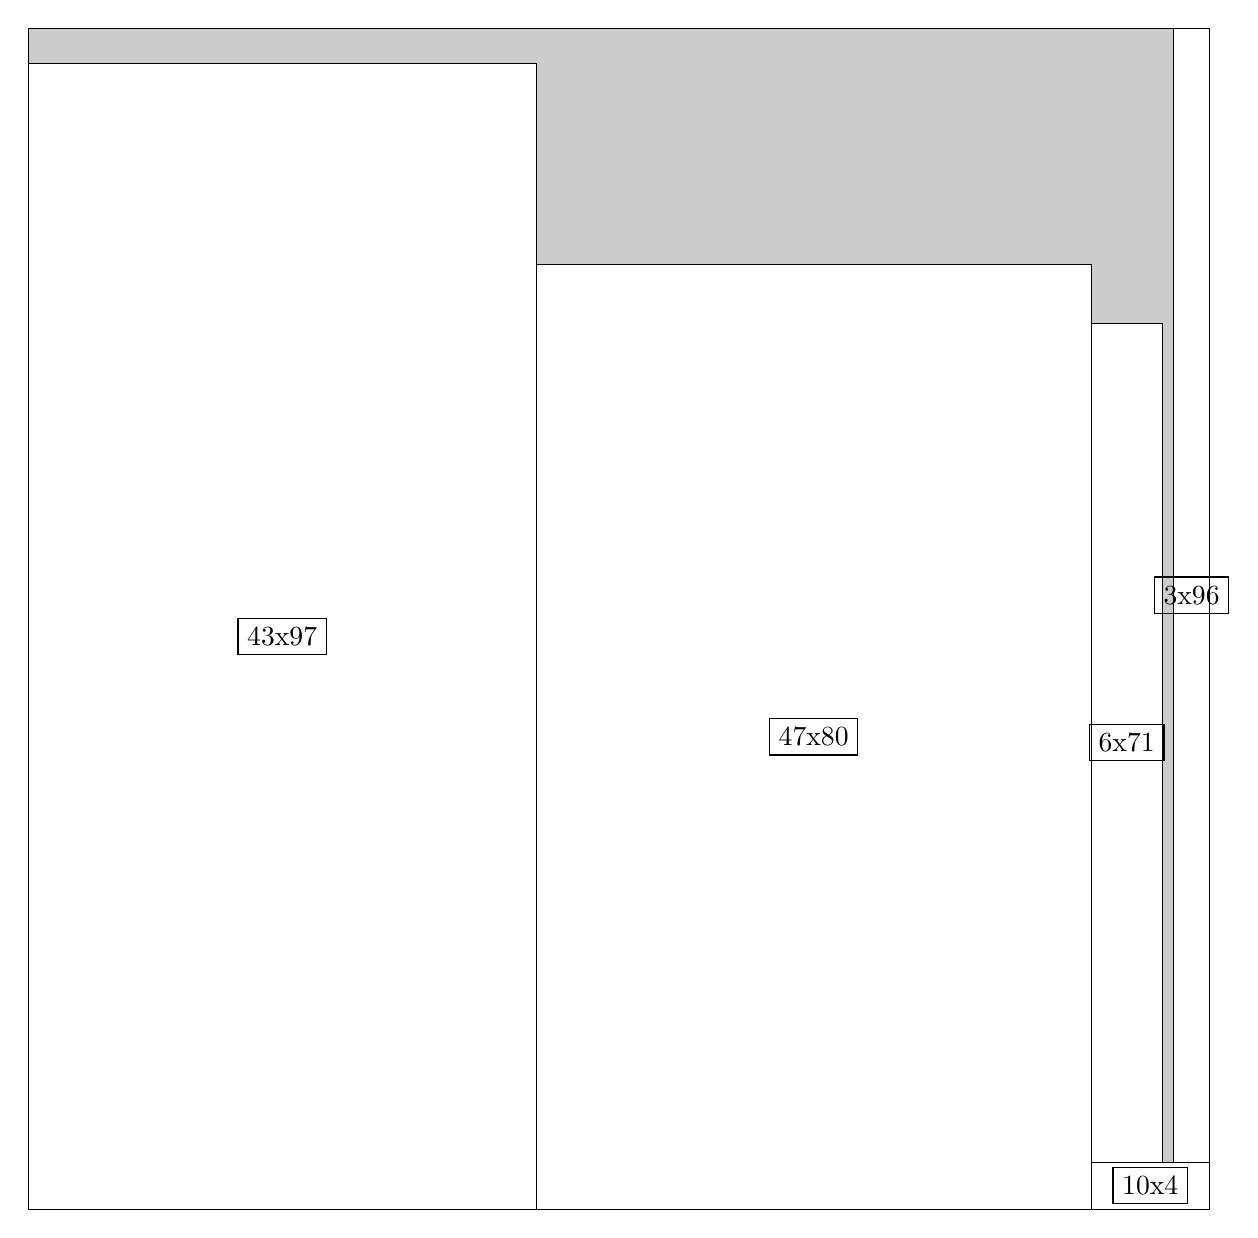
\begin{tikzpicture}[shorten >=1pt,scale=1.0,every node/.style={scale=1.0},->]
\tikzstyle{vertex}=[circle,fill=black!25,minimum size=14pt,inner sep=0pt]
\filldraw[fill=gray!40!white, draw=black] (0,0) rectangle (15.0,15.0);
\foreach \name/\x/\y/\w/\h in {43x97/0.0/0.0/6.45/14.549999999999999,47x80/6.45/0.0/7.05/12.0,6x71/13.5/0.6/0.8999999999999999/10.65,3x96/14.549999999999999/0.6/0.44999999999999996/14.399999999999999,10x4/13.5/0.0/1.5/0.6}
\filldraw[fill=white!40!white, draw=black] (\x,\y) rectangle node[draw] (\name) {\name} ++(\w,\h);
\end{tikzpicture}


w =43 , h =97 , x =0 , y =0 , v =4171
\par
w =47 , h =80 , x =43 , y =0 , v =3760
\par
w =6 , h =71 , x =90 , y =4 , v =426
\par
w =3 , h =96 , x =97 , y =4 , v =288
\par
w =10 , h =4 , x =90 , y =0 , v =40
\par
\newpage


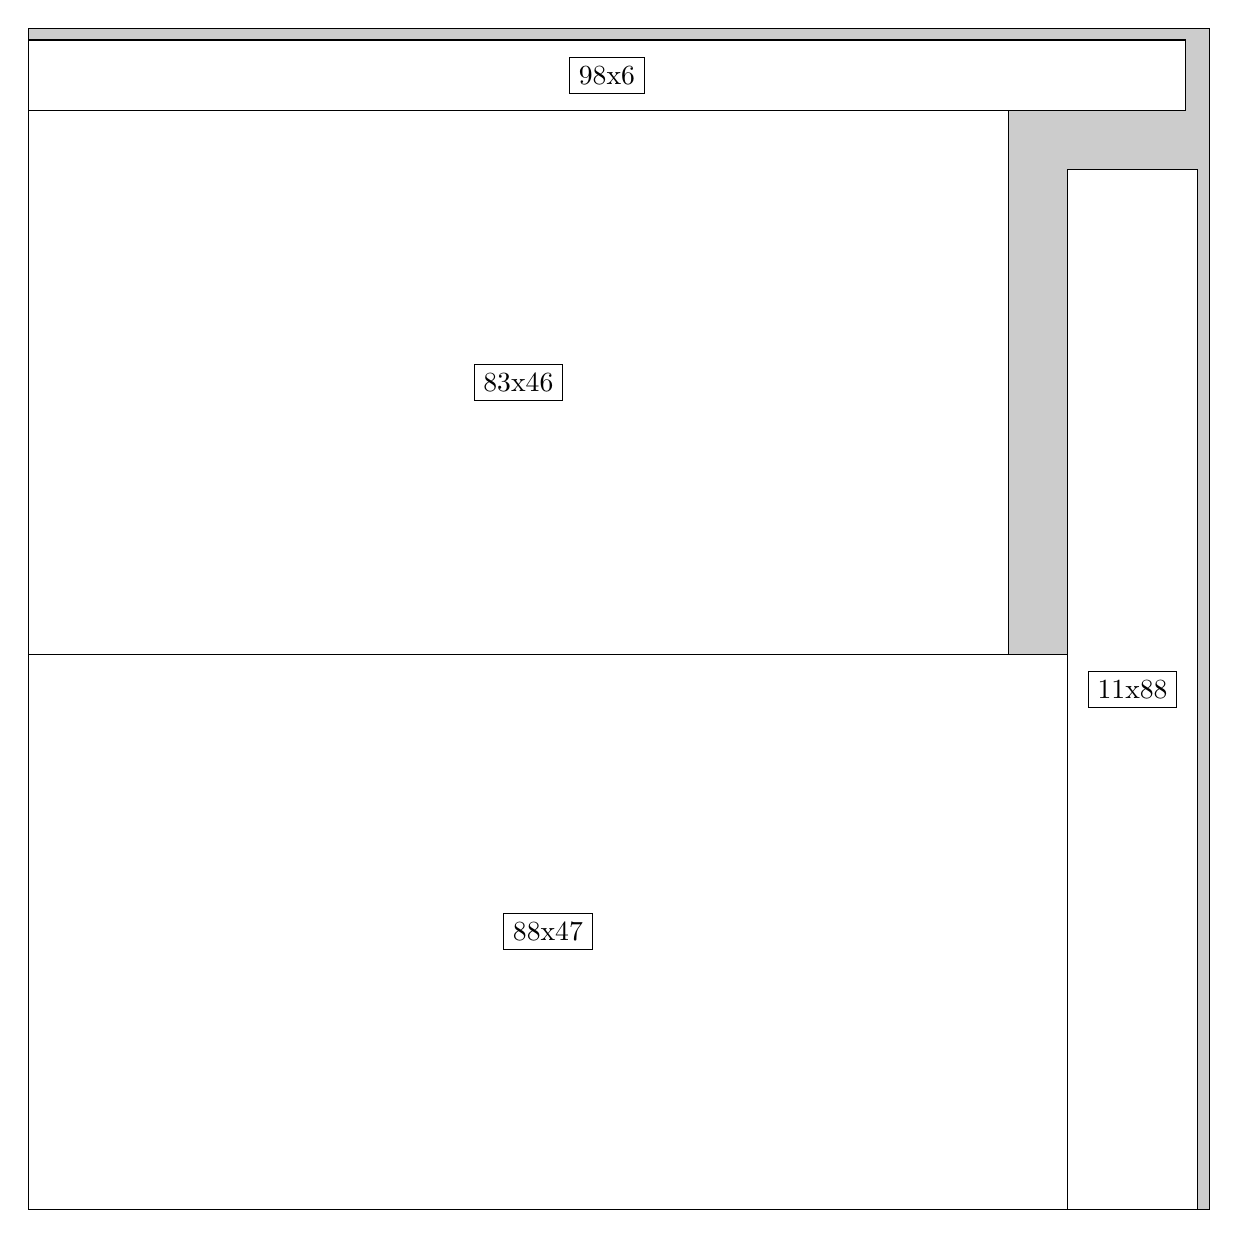
\begin{tikzpicture}[shorten >=1pt,scale=1.0,every node/.style={scale=1.0},->]
\tikzstyle{vertex}=[circle,fill=black!25,minimum size=14pt,inner sep=0pt]
\filldraw[fill=gray!40!white, draw=black] (0,0) rectangle (15.0,15.0);
\foreach \name/\x/\y/\w/\h in {88x47/0.0/0.0/13.2/7.05,83x46/0.0/7.05/12.45/6.8999999999999995,11x88/13.2/0.0/1.65/13.2,98x6/0.0/13.95/14.7/0.8999999999999999}
\filldraw[fill=white!40!white, draw=black] (\x,\y) rectangle node[draw] (\name) {\name} ++(\w,\h);
\end{tikzpicture}


w =88 , h =47 , x =0 , y =0 , v =4136
\par
w =83 , h =46 , x =0 , y =47 , v =3818
\par
w =11 , h =88 , x =88 , y =0 , v =968
\par
w =98 , h =6 , x =0 , y =93 , v =588
\par
\newpage


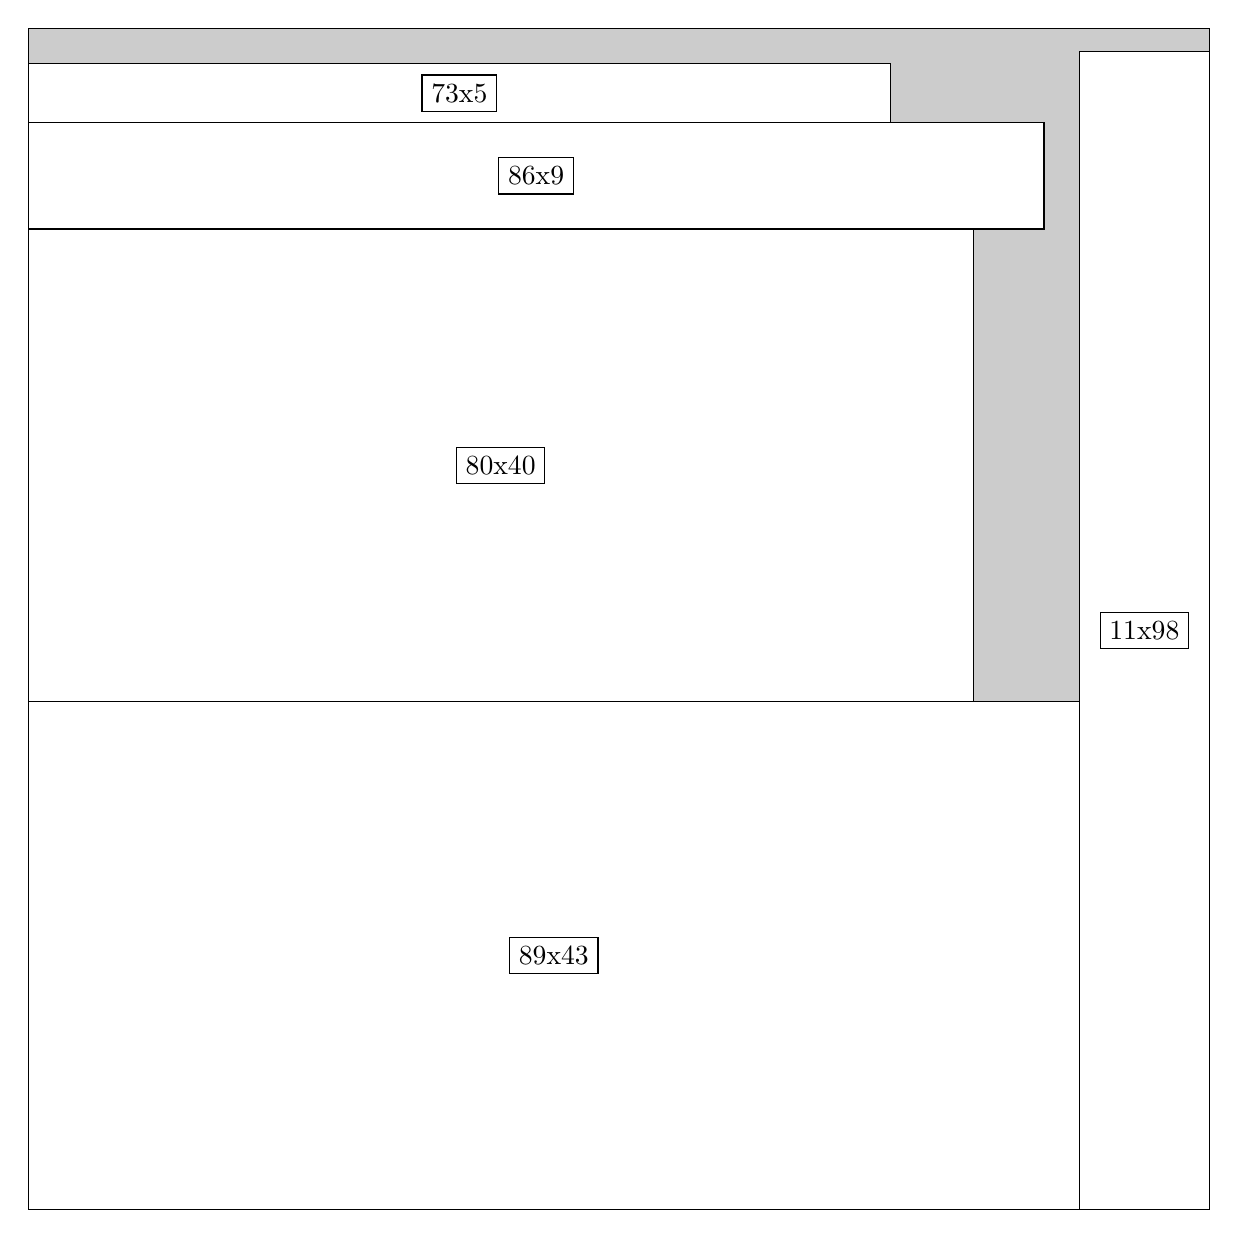
\begin{tikzpicture}[shorten >=1pt,scale=1.0,every node/.style={scale=1.0},->]
\tikzstyle{vertex}=[circle,fill=black!25,minimum size=14pt,inner sep=0pt]
\filldraw[fill=gray!40!white, draw=black] (0,0) rectangle (15.0,15.0);
\foreach \name/\x/\y/\w/\h in {89x43/0.0/0.0/13.35/6.45,80x40/0.0/6.45/12.0/6.0,11x98/13.35/0.0/1.65/14.7,86x9/0.0/12.45/12.9/1.3499999999999999,73x5/0.0/13.799999999999999/10.95/0.75}
\filldraw[fill=white!40!white, draw=black] (\x,\y) rectangle node[draw] (\name) {\name} ++(\w,\h);
\end{tikzpicture}


w =89 , h =43 , x =0 , y =0 , v =3827
\par
w =80 , h =40 , x =0 , y =43 , v =3200
\par
w =11 , h =98 , x =89 , y =0 , v =1078
\par
w =86 , h =9 , x =0 , y =83 , v =774
\par
w =73 , h =5 , x =0 , y =92 , v =365
\par
\newpage


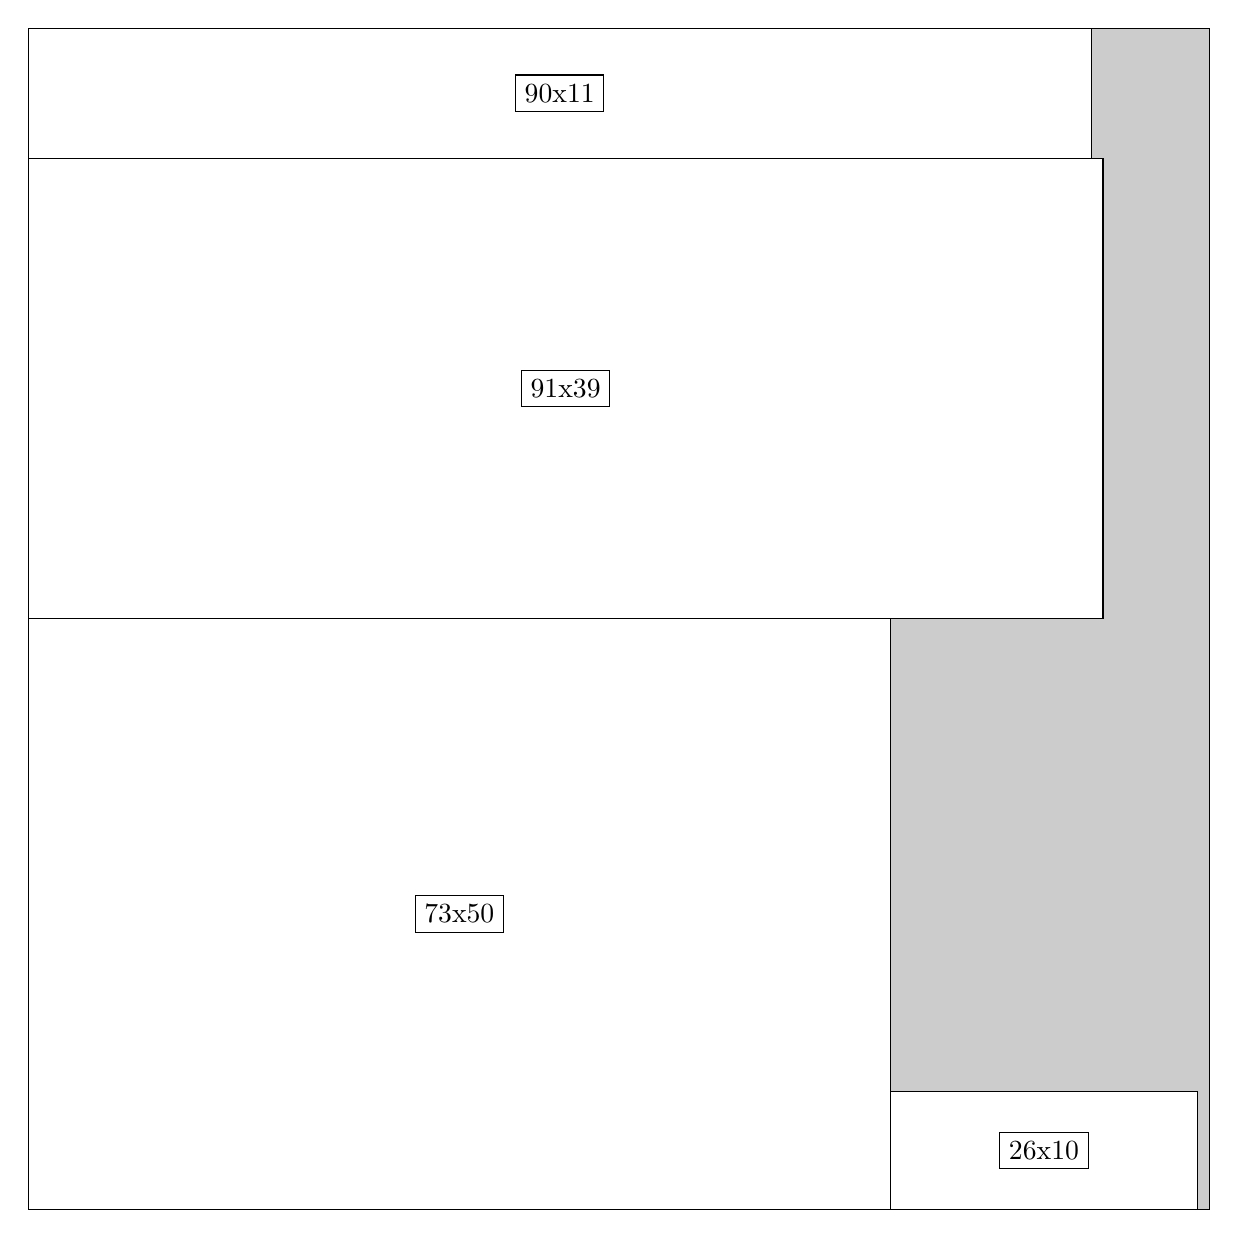
\begin{tikzpicture}[shorten >=1pt,scale=1.0,every node/.style={scale=1.0},->]
\tikzstyle{vertex}=[circle,fill=black!25,minimum size=14pt,inner sep=0pt]
\filldraw[fill=gray!40!white, draw=black] (0,0) rectangle (15.0,15.0);
\foreach \name/\x/\y/\w/\h in {73x50/0.0/0.0/10.95/7.5,91x39/0.0/7.5/13.65/5.85,90x11/0.0/13.35/13.5/1.65,26x10/10.95/0.0/3.9/1.5}
\filldraw[fill=white!40!white, draw=black] (\x,\y) rectangle node[draw] (\name) {\name} ++(\w,\h);
\end{tikzpicture}


w =73 , h =50 , x =0 , y =0 , v =3650
\par
w =91 , h =39 , x =0 , y =50 , v =3549
\par
w =90 , h =11 , x =0 , y =89 , v =990
\par
w =26 , h =10 , x =73 , y =0 , v =260
\par
\newpage


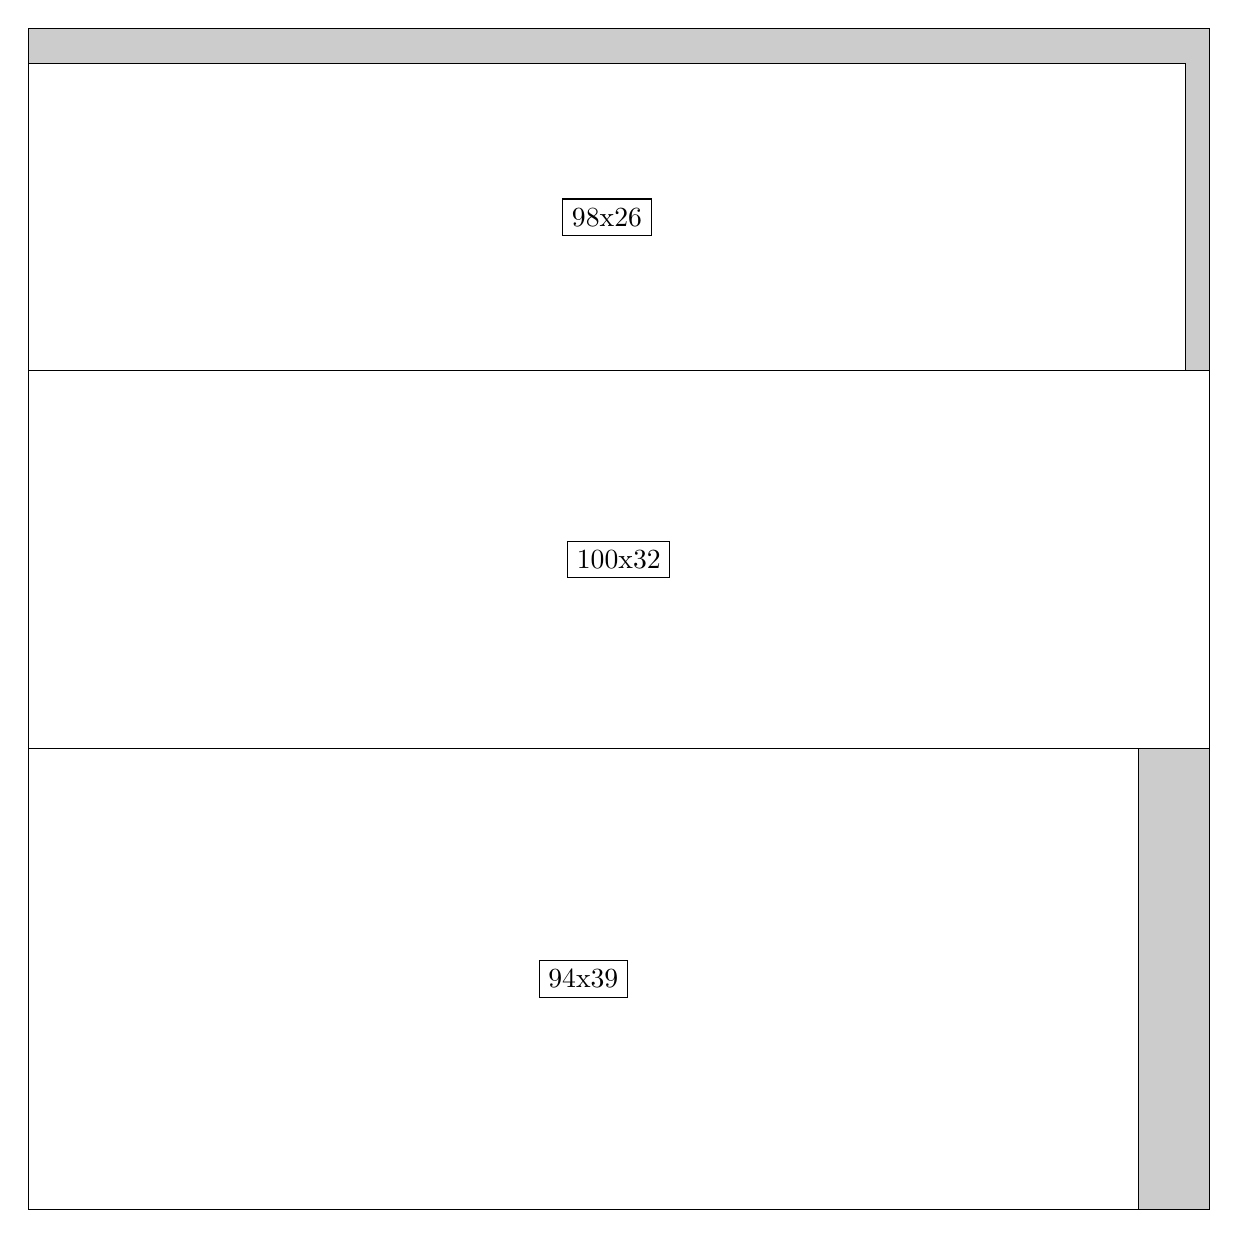
\begin{tikzpicture}[shorten >=1pt,scale=1.0,every node/.style={scale=1.0},->]
\tikzstyle{vertex}=[circle,fill=black!25,minimum size=14pt,inner sep=0pt]
\filldraw[fill=gray!40!white, draw=black] (0,0) rectangle (15.0,15.0);
\foreach \name/\x/\y/\w/\h in {94x39/0.0/0.0/14.1/5.85,100x32/0.0/5.85/15.0/4.8,98x26/0.0/10.65/14.7/3.9}
\filldraw[fill=white!40!white, draw=black] (\x,\y) rectangle node[draw] (\name) {\name} ++(\w,\h);
\end{tikzpicture}


w =94 , h =39 , x =0 , y =0 , v =3666
\par
w =100 , h =32 , x =0 , y =39 , v =3200
\par
w =98 , h =26 , x =0 , y =71 , v =2548
\par
\newpage


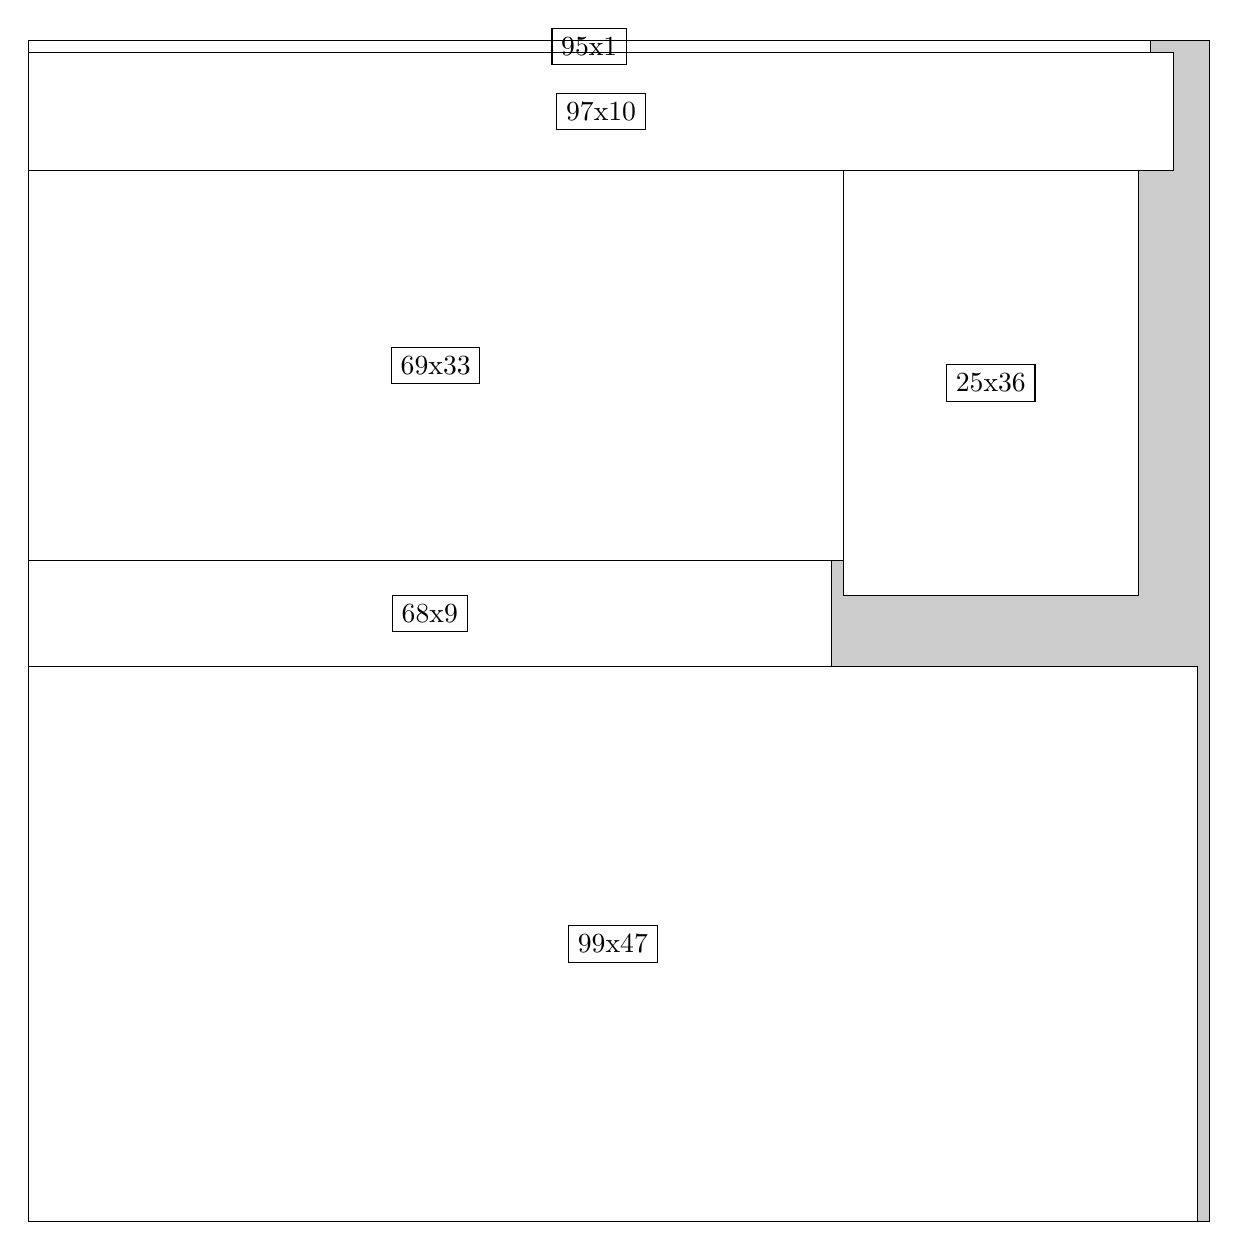
\begin{tikzpicture}[shorten >=1pt,scale=1.0,every node/.style={scale=1.0},->]
\tikzstyle{vertex}=[circle,fill=black!25,minimum size=14pt,inner sep=0pt]
\filldraw[fill=gray!40!white, draw=black] (0,0) rectangle (15.0,15.0);
\foreach \name/\x/\y/\w/\h in {99x47/0.0/0.0/14.85/7.05,68x9/0.0/7.05/10.2/1.3499999999999999,69x33/0.0/8.4/10.35/4.95,97x10/0.0/13.35/14.549999999999999/1.5,25x36/10.35/7.949999999999999/3.75/5.3999999999999995,95x1/0.0/14.85/14.25/0.15}
\filldraw[fill=white!40!white, draw=black] (\x,\y) rectangle node[draw] (\name) {\name} ++(\w,\h);
\end{tikzpicture}


w =99 , h =47 , x =0 , y =0 , v =4653
\par
w =68 , h =9 , x =0 , y =47 , v =612
\par
w =69 , h =33 , x =0 , y =56 , v =2277
\par
w =97 , h =10 , x =0 , y =89 , v =970
\par
w =25 , h =36 , x =69 , y =53 , v =900
\par
w =95 , h =1 , x =0 , y =99 , v =95
\par
\newpage


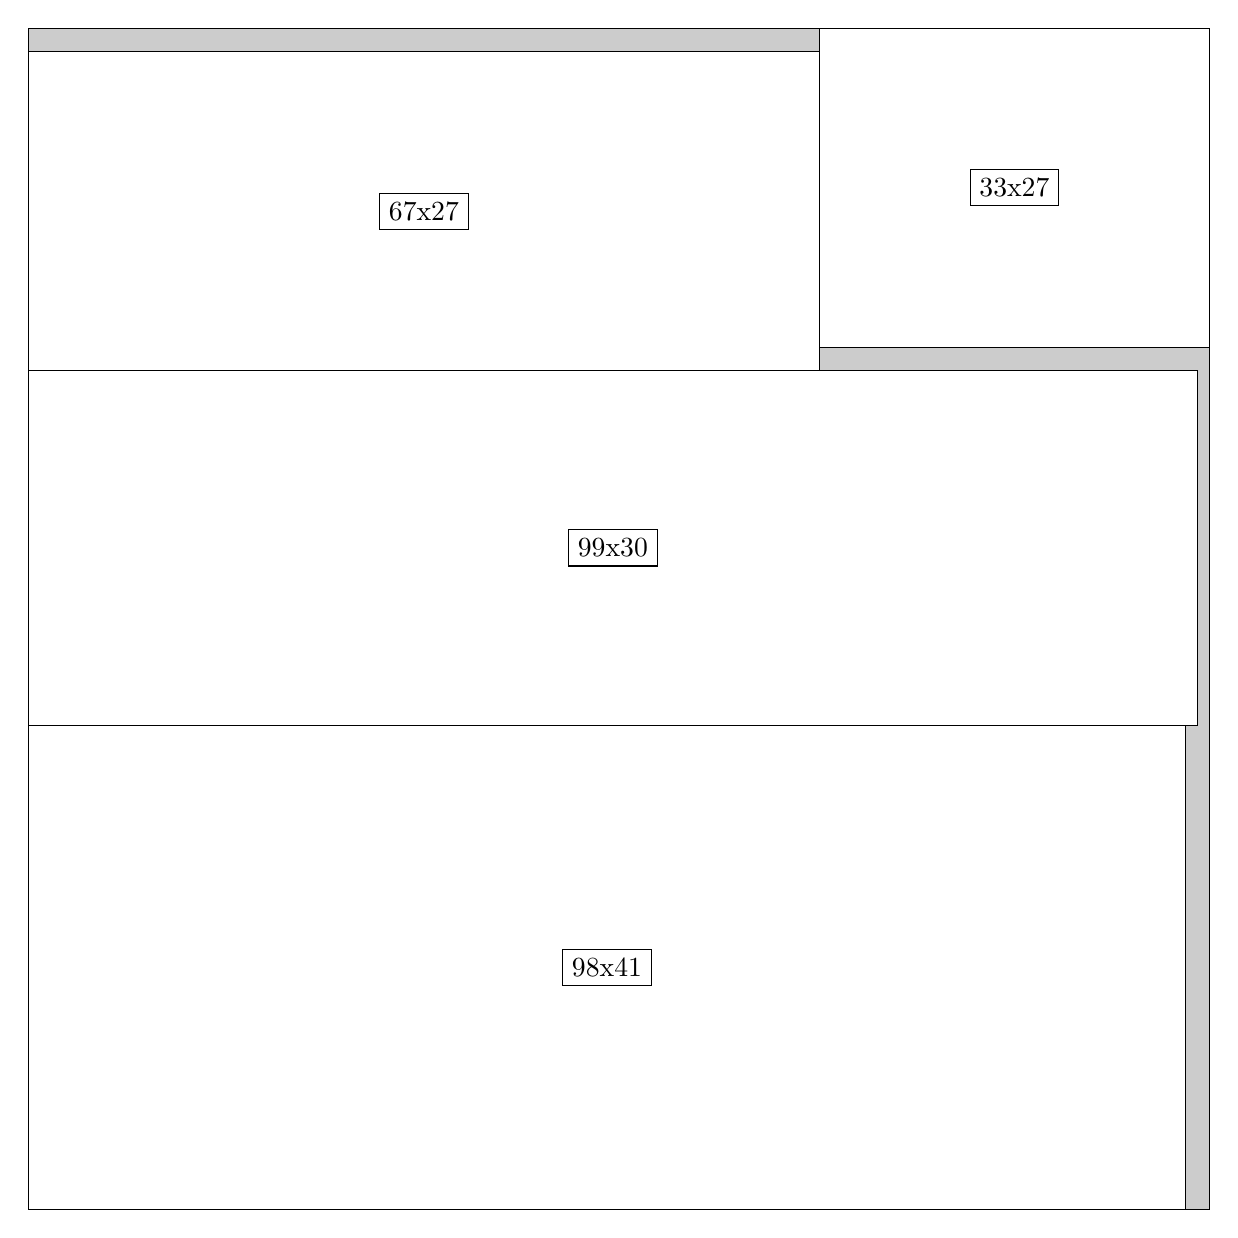
\begin{tikzpicture}[shorten >=1pt,scale=1.0,every node/.style={scale=1.0},->]
\tikzstyle{vertex}=[circle,fill=black!25,minimum size=14pt,inner sep=0pt]
\filldraw[fill=gray!40!white, draw=black] (0,0) rectangle (15.0,15.0);
\foreach \name/\x/\y/\w/\h in {98x41/0.0/0.0/14.7/6.1499999999999995,99x30/0.0/6.1499999999999995/14.85/4.5,67x27/0.0/10.65/10.049999999999999/4.05,33x27/10.049999999999999/10.95/4.95/4.05}
\filldraw[fill=white!40!white, draw=black] (\x,\y) rectangle node[draw] (\name) {\name} ++(\w,\h);
\end{tikzpicture}


w =98 , h =41 , x =0 , y =0 , v =4018
\par
w =99 , h =30 , x =0 , y =41 , v =2970
\par
w =67 , h =27 , x =0 , y =71 , v =1809
\par
w =33 , h =27 , x =67 , y =73 , v =891
\par
\newpage


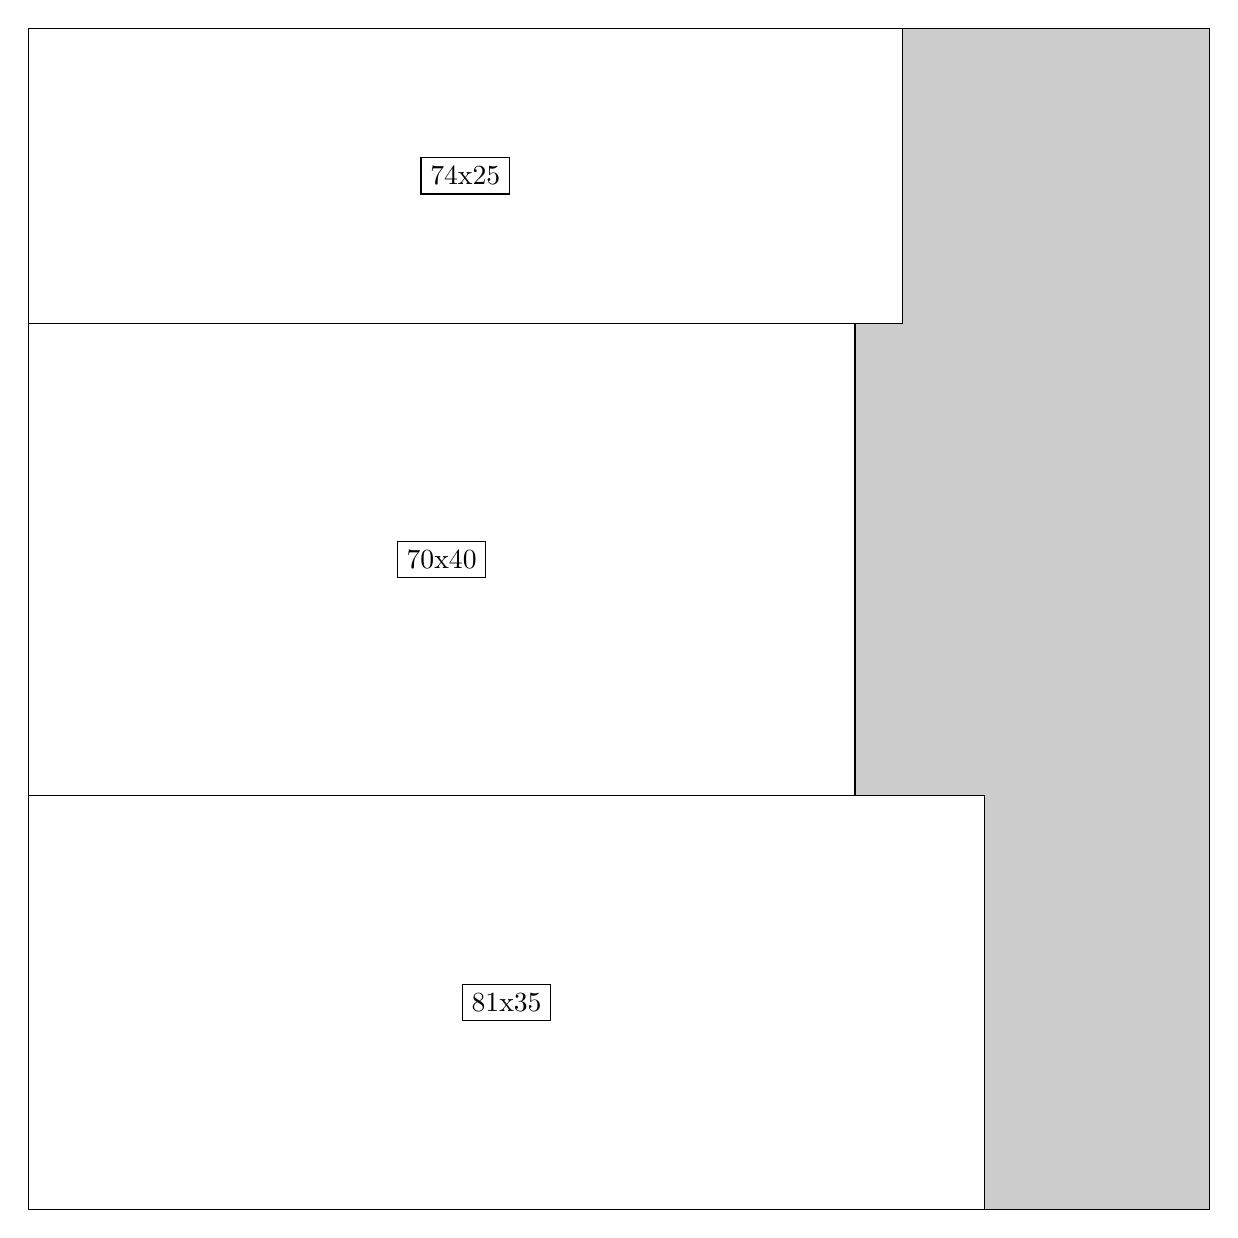
\begin{tikzpicture}[shorten >=1pt,scale=1.0,every node/.style={scale=1.0},->]
\tikzstyle{vertex}=[circle,fill=black!25,minimum size=14pt,inner sep=0pt]
\filldraw[fill=gray!40!white, draw=black] (0,0) rectangle (15.0,15.0);
\foreach \name/\x/\y/\w/\h in {81x35/0.0/0.0/12.15/5.25,70x40/0.0/5.25/10.5/6.0,74x25/0.0/11.25/11.1/3.75}
\filldraw[fill=white!40!white, draw=black] (\x,\y) rectangle node[draw] (\name) {\name} ++(\w,\h);
\end{tikzpicture}


w =81 , h =35 , x =0 , y =0 , v =2835
\par
w =70 , h =40 , x =0 , y =35 , v =2800
\par
w =74 , h =25 , x =0 , y =75 , v =1850
\par
\newpage


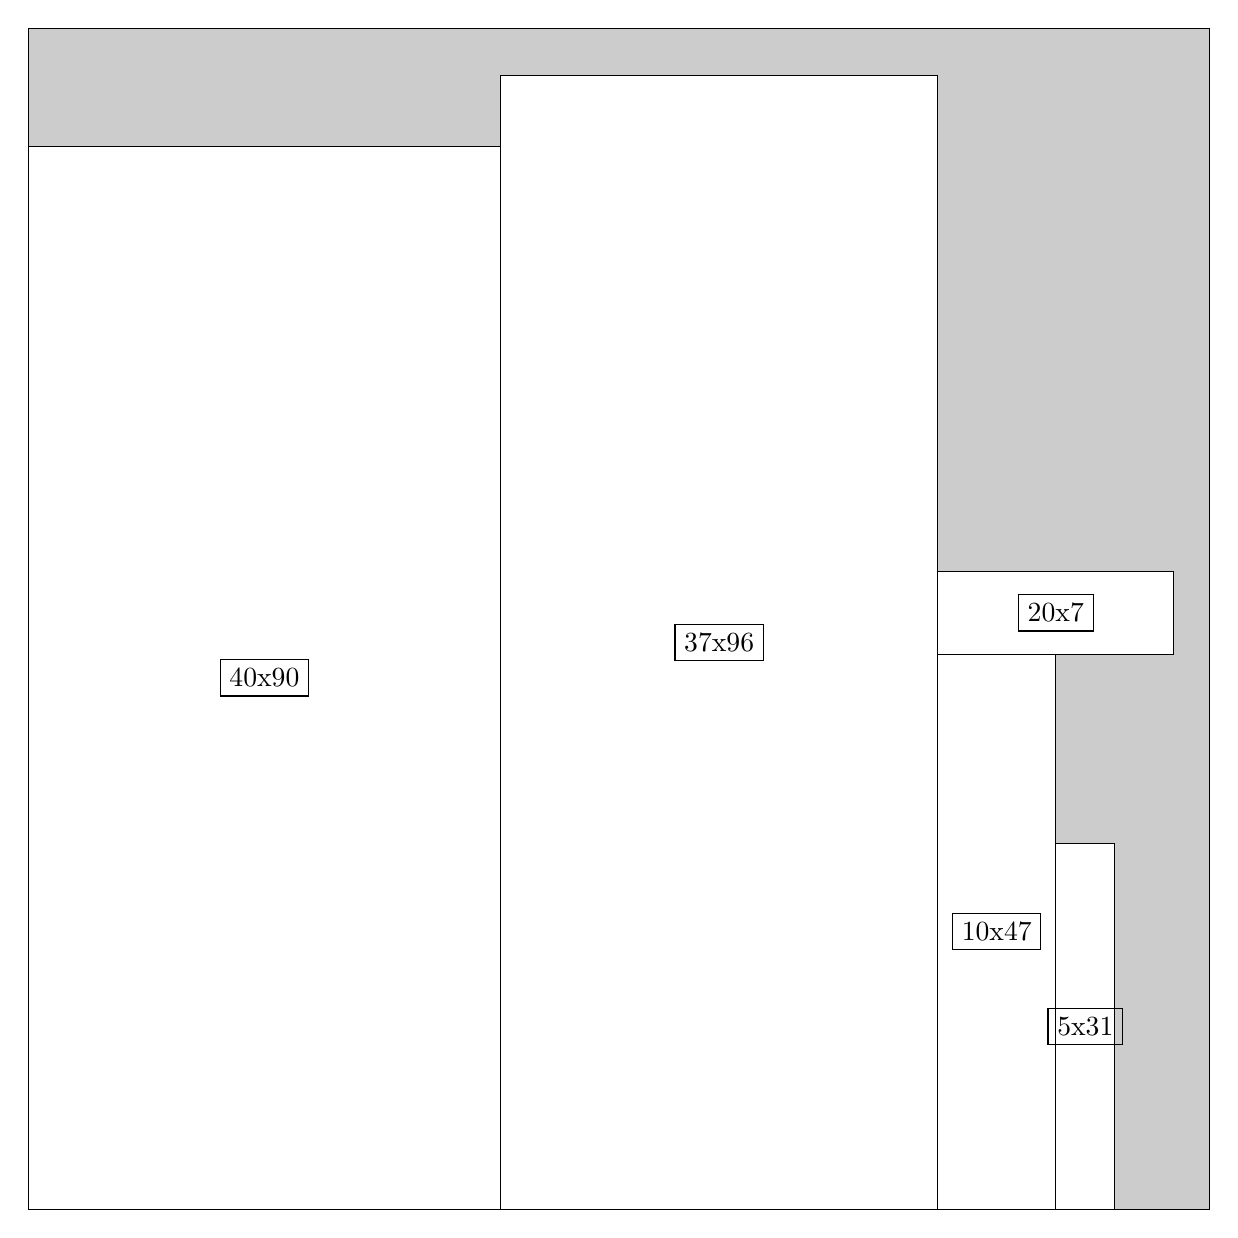
\begin{tikzpicture}[shorten >=1pt,scale=1.0,every node/.style={scale=1.0},->]
\tikzstyle{vertex}=[circle,fill=black!25,minimum size=14pt,inner sep=0pt]
\filldraw[fill=gray!40!white, draw=black] (0,0) rectangle (15.0,15.0);
\foreach \name/\x/\y/\w/\h in {40x90/0.0/0.0/6.0/13.5,37x96/6.0/0.0/5.55/14.399999999999999,10x47/11.549999999999999/0.0/1.5/7.05,5x31/13.049999999999999/0.0/0.75/4.6499999999999995,20x7/11.549999999999999/7.05/3.0/1.05}
\filldraw[fill=white!40!white, draw=black] (\x,\y) rectangle node[draw] (\name) {\name} ++(\w,\h);
\end{tikzpicture}


w =40 , h =90 , x =0 , y =0 , v =3600
\par
w =37 , h =96 , x =40 , y =0 , v =3552
\par
w =10 , h =47 , x =77 , y =0 , v =470
\par
w =5 , h =31 , x =87 , y =0 , v =155
\par
w =20 , h =7 , x =77 , y =47 , v =140
\par
\newpage


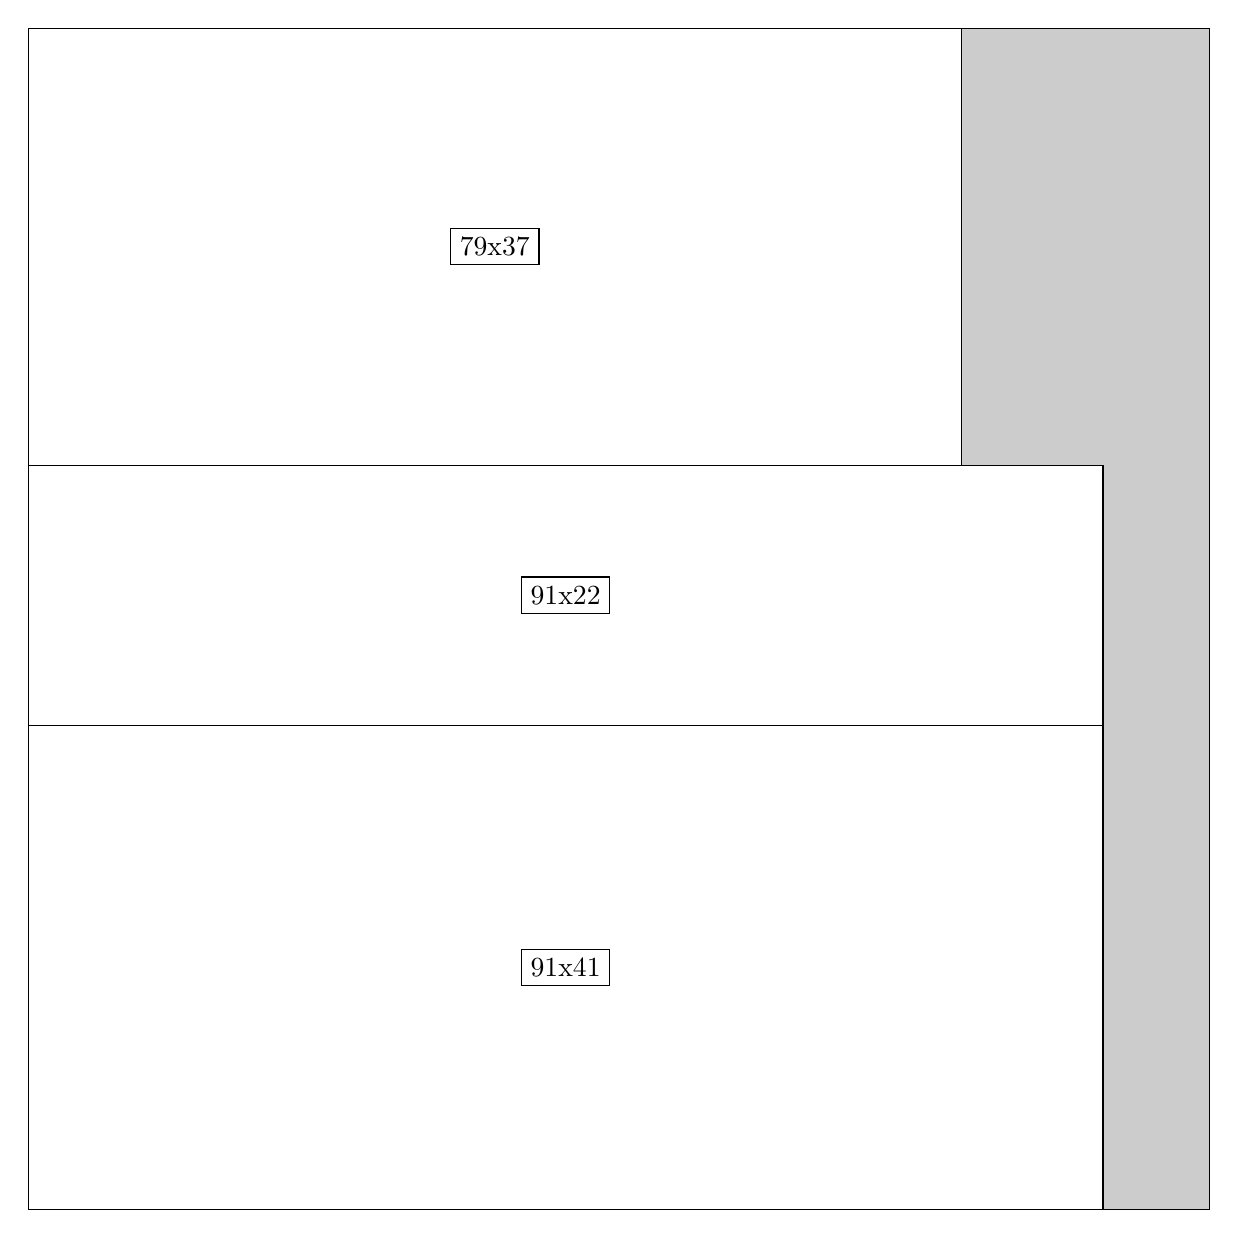
\begin{tikzpicture}[shorten >=1pt,scale=1.0,every node/.style={scale=1.0},->]
\tikzstyle{vertex}=[circle,fill=black!25,minimum size=14pt,inner sep=0pt]
\filldraw[fill=gray!40!white, draw=black] (0,0) rectangle (15.0,15.0);
\foreach \name/\x/\y/\w/\h in {91x41/0.0/0.0/13.65/6.1499999999999995,79x37/0.0/9.45/11.85/5.55,91x22/0.0/6.1499999999999995/13.65/3.3}
\filldraw[fill=white!40!white, draw=black] (\x,\y) rectangle node[draw] (\name) {\name} ++(\w,\h);
\end{tikzpicture}


w =91 , h =41 , x =0 , y =0 , v =3731
\par
w =79 , h =37 , x =0 , y =63 , v =2923
\par
w =91 , h =22 , x =0 , y =41 , v =2002
\par
\newpage


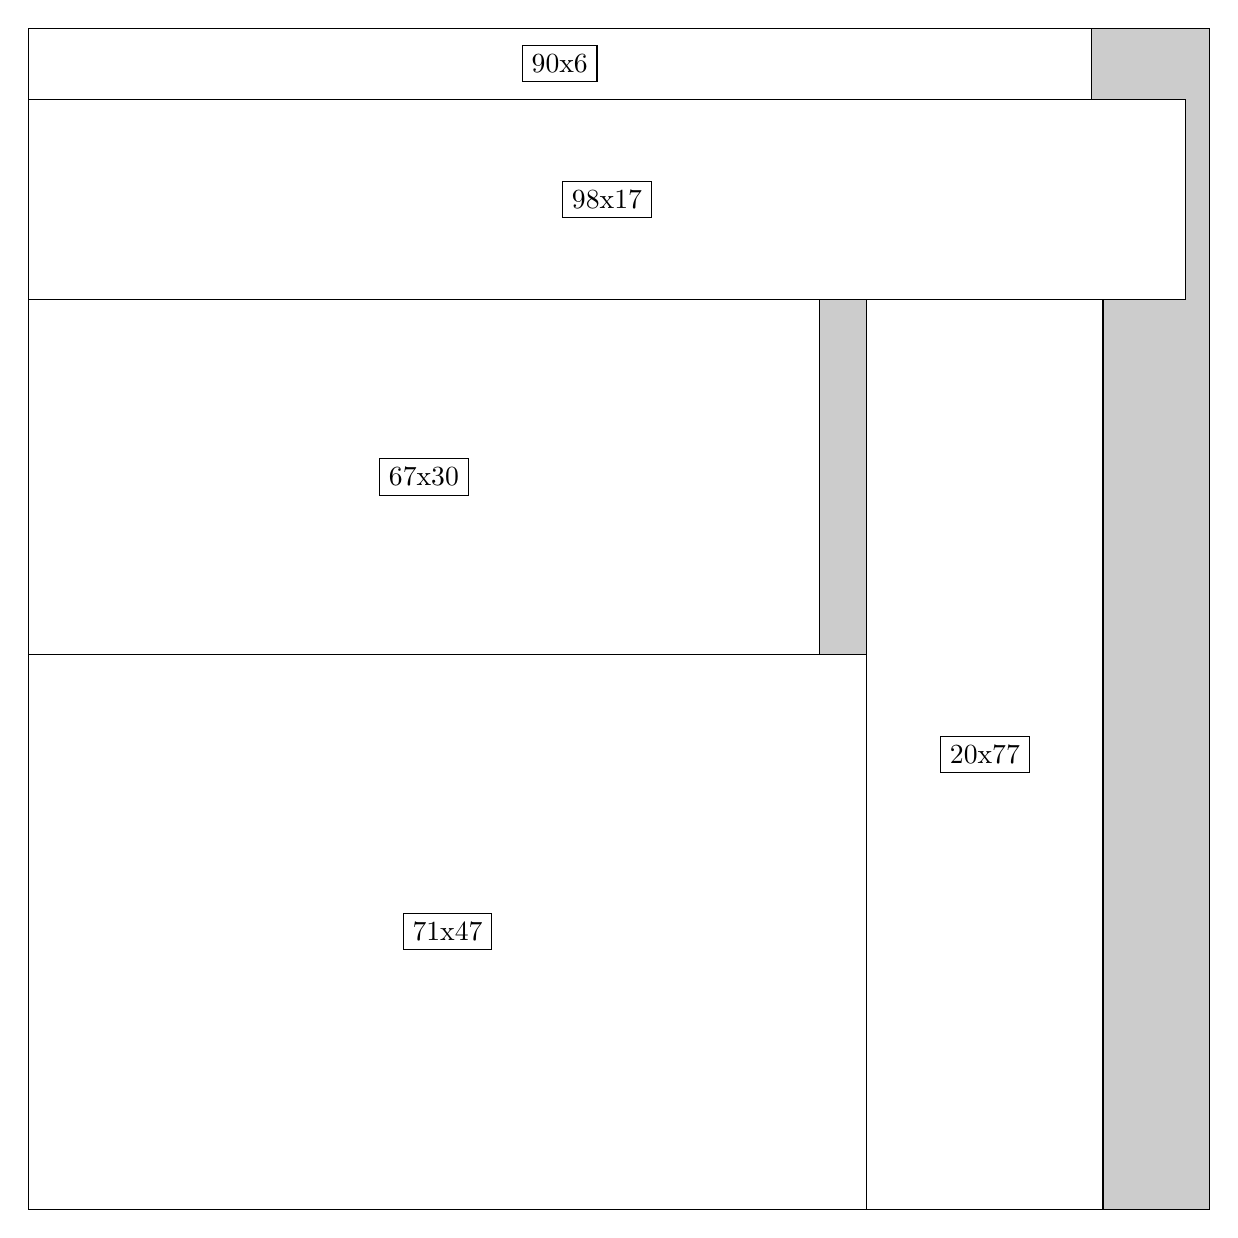
\begin{tikzpicture}[shorten >=1pt,scale=1.0,every node/.style={scale=1.0},->]
\tikzstyle{vertex}=[circle,fill=black!25,minimum size=14pt,inner sep=0pt]
\filldraw[fill=gray!40!white, draw=black] (0,0) rectangle (15.0,15.0);
\foreach \name/\x/\y/\w/\h in {71x47/0.0/0.0/10.65/7.05,67x30/0.0/7.05/10.049999999999999/4.5,98x17/0.0/11.549999999999999/14.7/2.55,20x77/10.65/0.0/3.0/11.549999999999999,90x6/0.0/14.1/13.5/0.8999999999999999}
\filldraw[fill=white!40!white, draw=black] (\x,\y) rectangle node[draw] (\name) {\name} ++(\w,\h);
\end{tikzpicture}


w =71 , h =47 , x =0 , y =0 , v =3337
\par
w =67 , h =30 , x =0 , y =47 , v =2010
\par
w =98 , h =17 , x =0 , y =77 , v =1666
\par
w =20 , h =77 , x =71 , y =0 , v =1540
\par
w =90 , h =6 , x =0 , y =94 , v =540
\par
\newpage


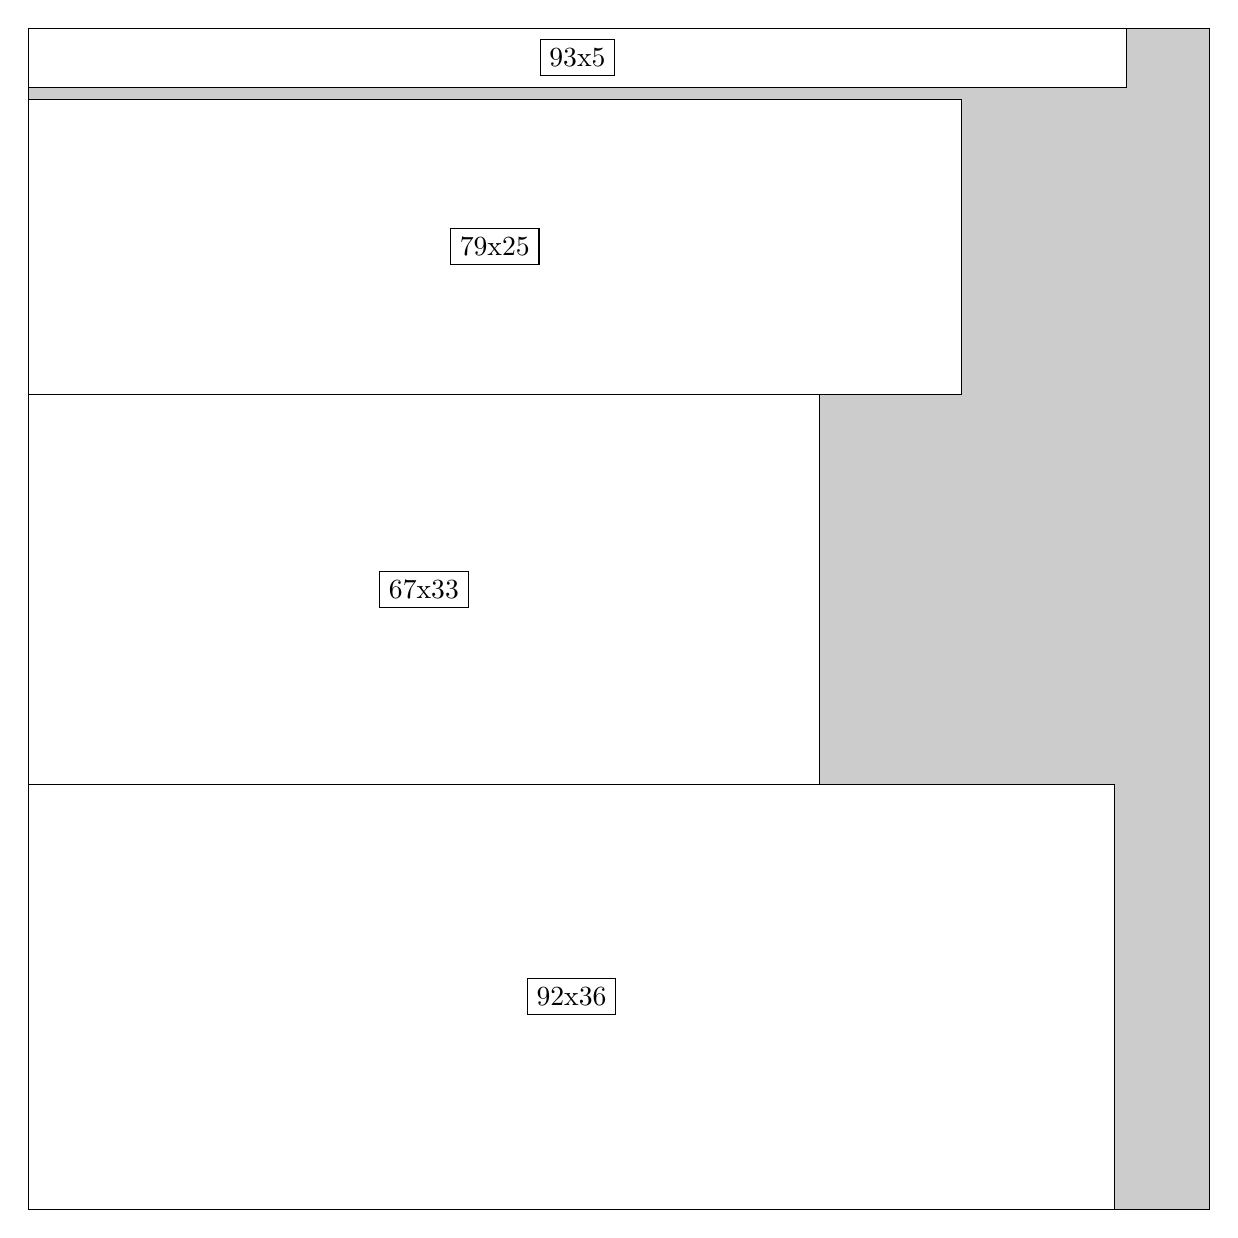
\begin{tikzpicture}[shorten >=1pt,scale=1.0,every node/.style={scale=1.0},->]
\tikzstyle{vertex}=[circle,fill=black!25,minimum size=14pt,inner sep=0pt]
\filldraw[fill=gray!40!white, draw=black] (0,0) rectangle (15.0,15.0);
\foreach \name/\x/\y/\w/\h in {92x36/0.0/0.0/13.799999999999999/5.3999999999999995,67x33/0.0/5.3999999999999995/10.049999999999999/4.95,79x25/0.0/10.35/11.85/3.75,93x5/0.0/14.25/13.95/0.75}
\filldraw[fill=white!40!white, draw=black] (\x,\y) rectangle node[draw] (\name) {\name} ++(\w,\h);
\end{tikzpicture}


w =92 , h =36 , x =0 , y =0 , v =3312
\par
w =67 , h =33 , x =0 , y =36 , v =2211
\par
w =79 , h =25 , x =0 , y =69 , v =1975
\par
w =93 , h =5 , x =0 , y =95 , v =465
\par
\newpage


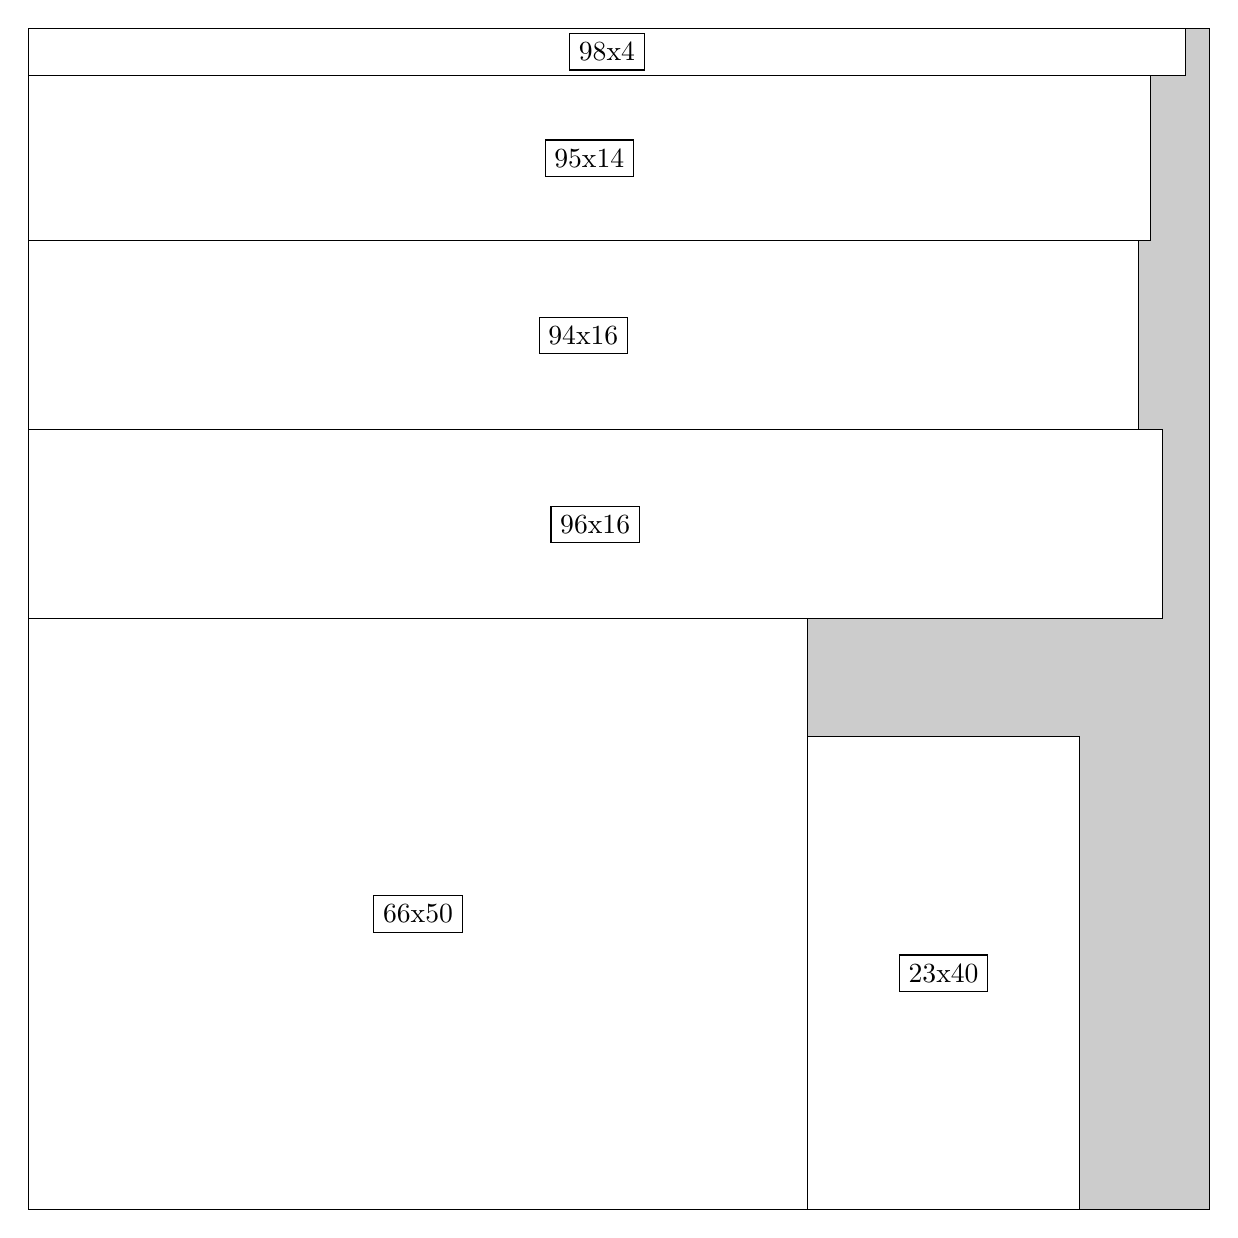
\begin{tikzpicture}[shorten >=1pt,scale=1.0,every node/.style={scale=1.0},->]
\tikzstyle{vertex}=[circle,fill=black!25,minimum size=14pt,inner sep=0pt]
\filldraw[fill=gray!40!white, draw=black] (0,0) rectangle (15.0,15.0);
\foreach \name/\x/\y/\w/\h in {66x50/0.0/0.0/9.9/7.5,96x16/0.0/7.5/14.399999999999999/2.4,94x16/0.0/9.9/14.1/2.4,95x14/0.0/12.299999999999999/14.25/2.1,23x40/9.9/0.0/3.4499999999999997/6.0,98x4/0.0/14.399999999999999/14.7/0.6}
\filldraw[fill=white!40!white, draw=black] (\x,\y) rectangle node[draw] (\name) {\name} ++(\w,\h);
\end{tikzpicture}


w =66 , h =50 , x =0 , y =0 , v =3300
\par
w =96 , h =16 , x =0 , y =50 , v =1536
\par
w =94 , h =16 , x =0 , y =66 , v =1504
\par
w =95 , h =14 , x =0 , y =82 , v =1330
\par
w =23 , h =40 , x =66 , y =0 , v =920
\par
w =98 , h =4 , x =0 , y =96 , v =392
\par
\newpage


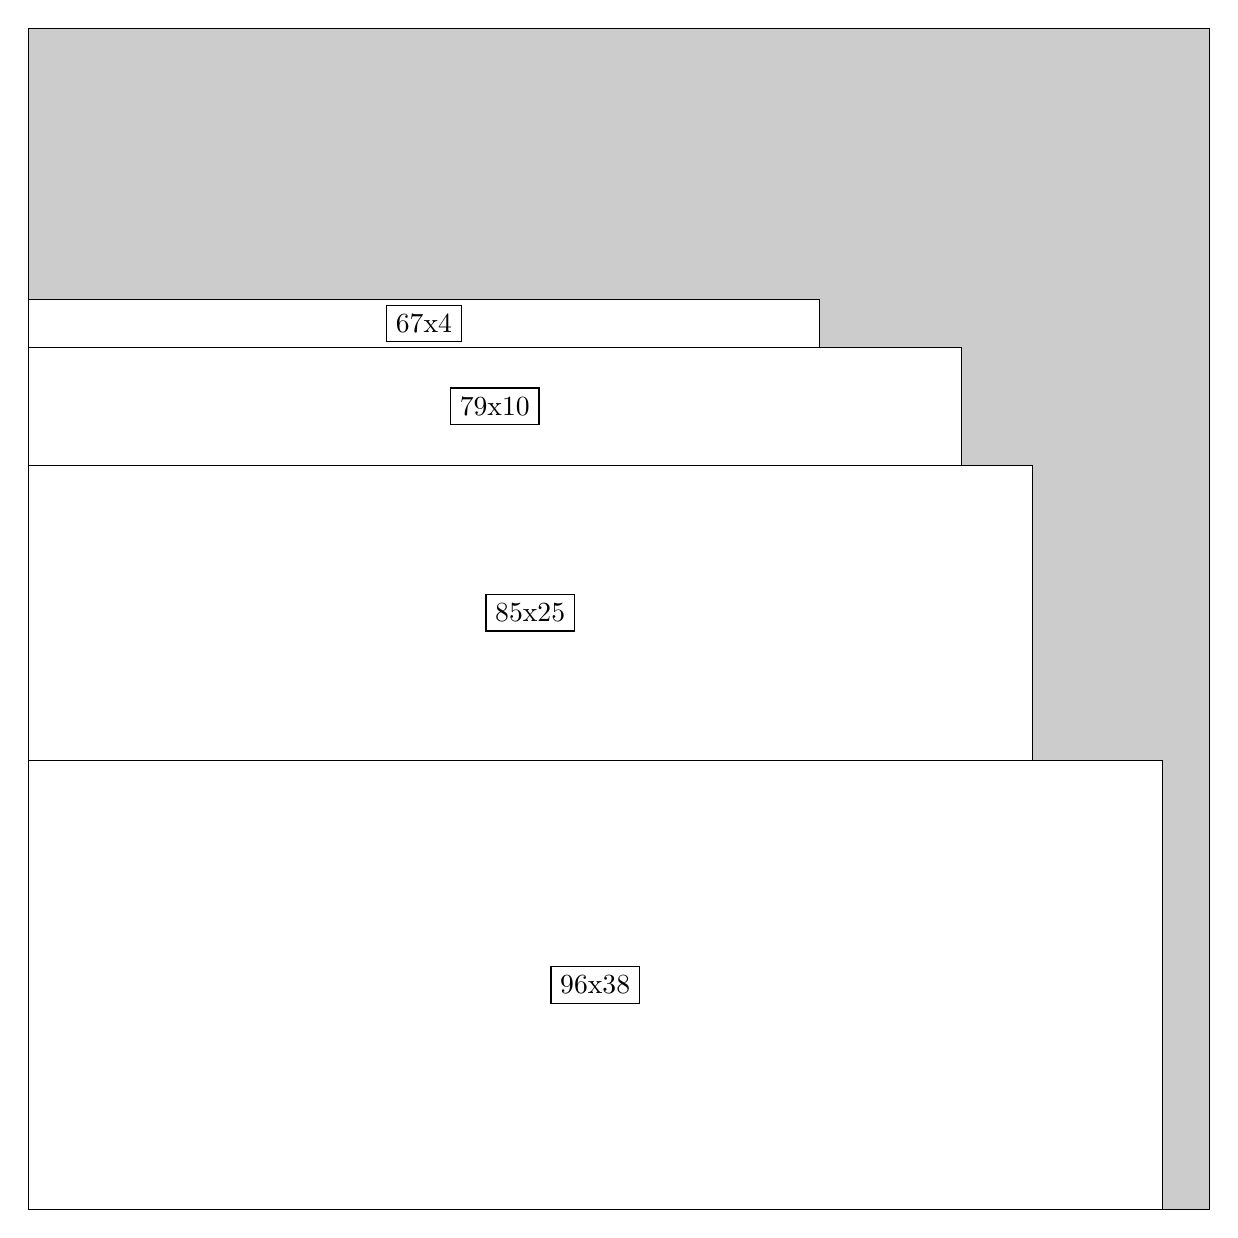
\begin{tikzpicture}[shorten >=1pt,scale=1.0,every node/.style={scale=1.0},->]
\tikzstyle{vertex}=[circle,fill=black!25,minimum size=14pt,inner sep=0pt]
\filldraw[fill=gray!40!white, draw=black] (0,0) rectangle (15.0,15.0);
\foreach \name/\x/\y/\w/\h in {96x38/0.0/0.0/14.399999999999999/5.7,85x25/0.0/5.7/12.75/3.75,79x10/0.0/9.45/11.85/1.5,67x4/0.0/10.95/10.049999999999999/0.6}
\filldraw[fill=white!40!white, draw=black] (\x,\y) rectangle node[draw] (\name) {\name} ++(\w,\h);
\end{tikzpicture}


w =96 , h =38 , x =0 , y =0 , v =3648
\par
w =85 , h =25 , x =0 , y =38 , v =2125
\par
w =79 , h =10 , x =0 , y =63 , v =790
\par
w =67 , h =4 , x =0 , y =73 , v =268
\par
\newpage


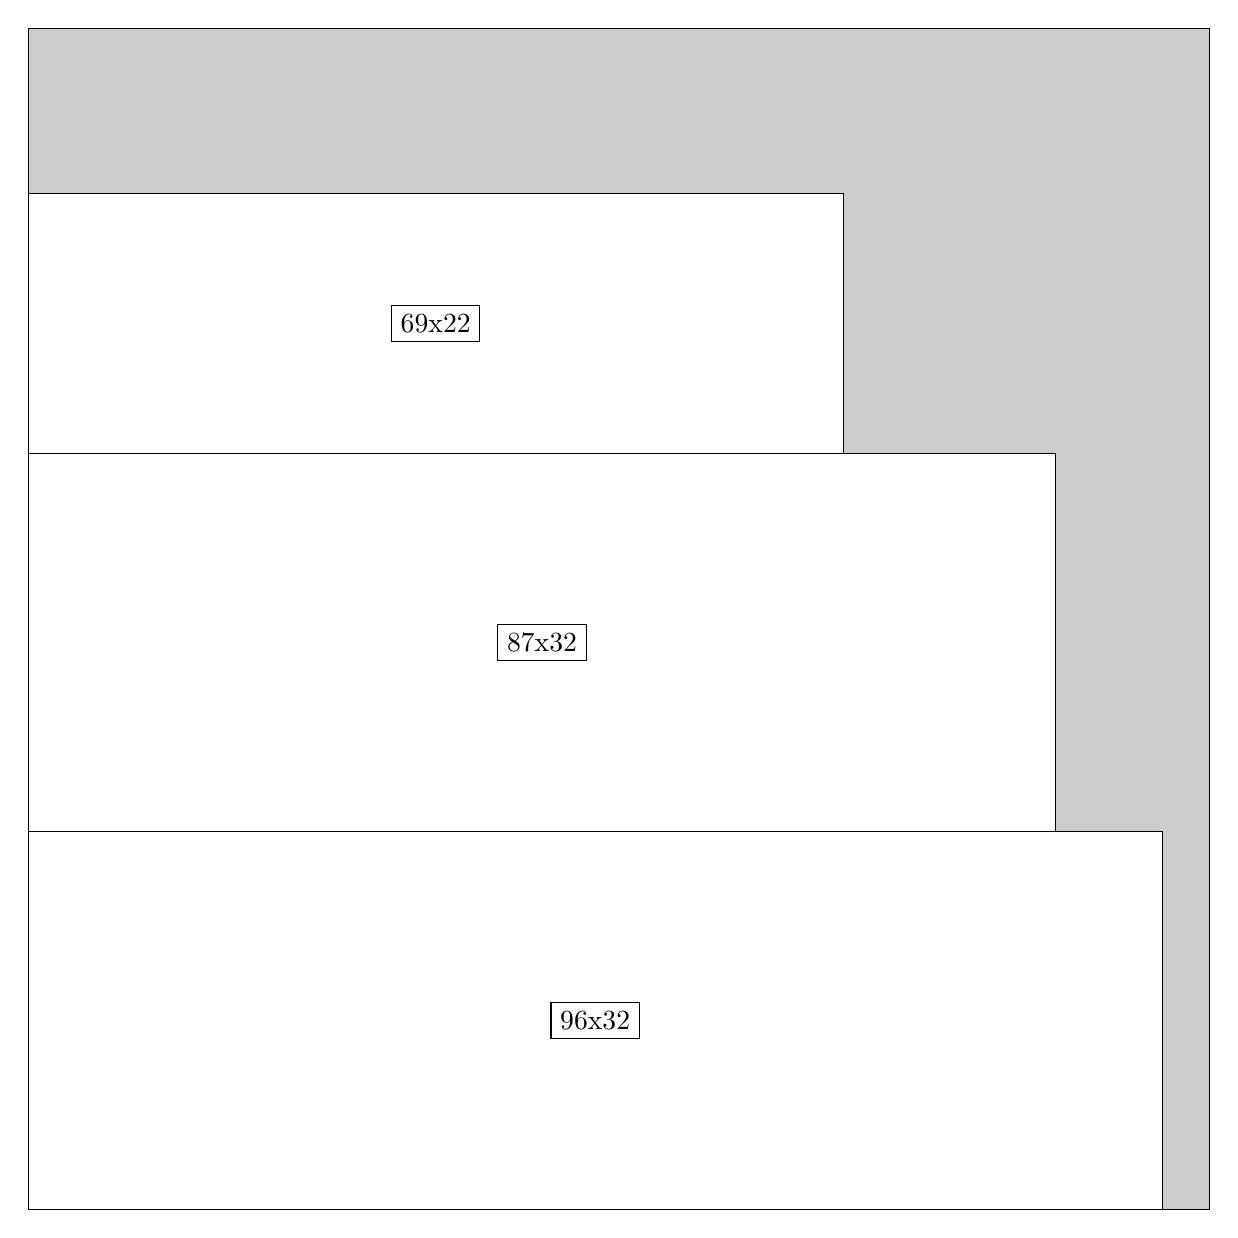
\begin{tikzpicture}[shorten >=1pt,scale=1.0,every node/.style={scale=1.0},->]
\tikzstyle{vertex}=[circle,fill=black!25,minimum size=14pt,inner sep=0pt]
\filldraw[fill=gray!40!white, draw=black] (0,0) rectangle (15.0,15.0);
\foreach \name/\x/\y/\w/\h in {96x32/0.0/0.0/14.399999999999999/4.8,87x32/0.0/4.8/13.049999999999999/4.8,69x22/0.0/9.6/10.35/3.3}
\filldraw[fill=white!40!white, draw=black] (\x,\y) rectangle node[draw] (\name) {\name} ++(\w,\h);
\end{tikzpicture}


w =96 , h =32 , x =0 , y =0 , v =3072
\par
w =87 , h =32 , x =0 , y =32 , v =2784
\par
w =69 , h =22 , x =0 , y =64 , v =1518
\par
\newpage


\end{document}